\documentclass[letterpaper,12pt]{article}

\usepackage{amsmath,amsfonts,mathtools}
\usepackage{amsthm}
\usepackage{amssymb}
\usepackage{graphicx}
\usepackage{hyperref}
\usepackage{enumitem}
\usepackage{float}
\usepackage{tikz}

% For displaying code
\usepackage{listings}
\usepackage{color}

\definecolor{dkgreen}{rgb}{0,0.6,0}
\definecolor{gray}{rgb}{0.5,0.5,0.5}
\definecolor{mauve}{rgb}{0.58,0,0.82}
\definecolor{orangered}{rgb}{1,0.27,0}

% Settings for displaying code
\lstset{language=python}

% Display tildes nicely
\lstset{
    literate={~} {$\sim$}{1}
}

\newcommand*{\lstitem}[1]{
  \setbox0\hbox{\lstinline{#1}}
  \item[\usebox0]
}

% Personal definitions
\newcommand{\lra}{\ensuremath{\longrightarrow{}}}
\newcommand{\vect}[1]{\mathbf{#1}}
\newcommand{\matr}[1]{\mathbf{#1}}
\newcommand{\norm}[1]{\left\lVert#1\right\rVert}
\newcommand{\abs}[1]{\lvert#1\rvert}
\newcommand*{\vertbar}{\rule[-1ex]{0.5pt}{2.5ex}} % for complicated matrices
\newcommand*{\horzbar}{\rule[.5ex]{2.5ex}{0.5pt}}
\renewcommand{\qedsymbol}{\rule{0.7em}{0.7em}}
\newcommand{\tabitem}{~~\llap{\textbullet}~~}

\makeatletter
\def\idots{\mathinner{\mkern1mu\raise\p@
\vbox{\kern7\p@\hbox{.}}\mkern2mu
\raise4\p@\hbox{.}\mkern2mu\raise7\p@\hbox{.}\mkern1mu}}
\makeatother

\DeclareMathOperator{\tr}{tr}
\DeclareMathOperator{\rank}{rank}
\DeclareMathOperator{\diag}{diag}

% Theorem commands
\newtheorem{lem}{Lemma}
\newtheorem{thm}{Theorem}
\newtheorem{defn}{Definition}

% Set spacing
\setenumerate{itemsep=1.5pt,parsep=1.5pt,topsep=0.5pt}
\setlist{itemsep=1.5pt,parsep=1.5pt,leftmargin=1pt}
\setitemize{itemsep=1.5pt,parsep=1.5pt,topsep=0.5pt}

% set 1" margins on 8.5" x 11" paper
% top left is measured from 1", 1"
\topmargin       0in
\oddsidemargin   0in
\evensidemargin  0in
\headheight      0in
\headsep         0in
\topskip         0in
\textheight      9in
\textwidth       6.5in

\begin{document}
\title{CS131 Notes}
\author{Sean Wu}
\date{\today}
\maketitle

\tableofcontents

\pagebreak

% set spacing
\setlength{\parindent}{0em}
\setlength{\parskip}{1em}

\section{Introduction}
\subsection{What is Computer Vision and why is it hard}

\begin{description}
 \item[Computer Vision]: extracting info from digital images OR developing algorithms to understand image content for other applications
\end{description}
\begin{itemize}
 \item Computer Vision is a hard interdisciplinary problem that is still unsolved
       \begin{itemize}
        \item Hard to convert data storing RGB values in many pixels to semantic info (ex. this blob of black pixels is a chair)
       \end{itemize}
 \item Vision (extracting meaningful info) is harder than 3D modelling
\end{itemize}

\subsection{Definition of Vision and Comparisons to Human Vision}
\begin{description}
 \item[sensing device]: captures details from a scene
 \item[interpreting device]: processes image from sensing device to extract meaning
\end{description}

\begin{itemize}
 \item Humans use eyes as sensing devices while computers use cameras
 \item For sensing devices, computer vision is actually better than human vision because cameras can see infrared, have longer range, and capture greater detail
 \item For interpreting devices, the human brain is way more advanced than computer systems
\end{itemize}

\subsection{Human Vision Strengths and Weaknesses}
\begin{itemize}
 \item Human vision evolved to quickly recognize danger for survival
 \item It is very fast \lra $\sim150$ ms to recognize an animal
 \item For speed, humans \textit{focus} only on ``relevant'' \textit{areas of interest}
 \item Thus, small signals/changes in the background can be difficult to detect and segment
 \item Humans also use \textit{context} to infer clues
       \begin{itemize}
        \item Used to determine next area of focus, when to expect certain objects in certain positions, and colour compensation in shadows
        \item However, context can be used to trick human vision
       \end{itemize}
 \item Context is very hard to include in computer vision
\end{itemize}

\subsection{Extracting info from images}

\begin{itemize}
 \item 2 types of info extracted in computer vision: \textbf{measurements} and \textbf{semantic info}
\end{itemize}

\subsubsection{Measurement in Vision}
\begin{itemize}
 \item Robots scan surroundings to make a map of its environment
 \item Stereo vision gives depth information (like 2 eyes) using triangulation
       \begin{itemize}
        \item Depth info represented as a depth map
       \end{itemize}
 \item With multiple viewpoints of an object, a 3D surface can be created (or even a 3D model)
\end{itemize}

\subsubsection{Obtaining Semantic Info from Vision}
\begin{itemize}
 \item Labelling objects (or scene)
 \item Recognizing people, actions, gestures, faces
\end{itemize}

\subsection{Applications of Computer Vision}
\begin{itemize}
 \item Video special effects
 \item 3D object modelling
 \item Scene recognition
 \item Face detection
       \begin{itemize}
        \item Note: face recognition is harder than face detection
       \end{itemize}
 \item Optical Character Recognition (OCR)
 \item Reverse image search
 \item Vision based interaction (ex. Microsoft Kinect)
 \item Augmented reality
 \item Virtual reality
\end{itemize}

\section{Linear Algebra Review}
\subsection{Vectors}
\begin{itemize}
 \item a \textit{column vector} $\vect{v} \in \mathbb{R}^{n \times 1}$ where
       \begin{align}
        \vect{v} & = \begin{bmatrix}
         v_{1}  \\
         v_{2}  \\
         \vdots \\
         v_{n}
        \end{bmatrix}
       \end{align}
 \item a \textit{row vector} $\vect{v}^T \in \mathbb{R}^{1 \times n}$ where
       \begin{align}
        \vect{v}^T = \begin{bmatrix}
         v_1 & v_2 & \dots & v_n
        \end{bmatrix}
       \end{align}
\end{itemize}

\begin{itemize}
 \item The transpose of a matrix/vector is denoted with a subscript $T$
 \item Note: with \lstinline{numpy} in \lstinline{python}, you can transpose a vector \lstinline{v} with \lstinline{v.T}
\end{itemize}

\begin{itemize}
 \item In 2D and 3D, vectors have a geometric interpretation as points
 \item Can also use vectors to represent pixels, gradients at an image keypoint, etc
 \item In this use case, vectors do not have a geometric interpretation, but calculations like ``distance'' are still useful
       \begin{itemize}
        \item The distance measures ``similarity'' between 2 vectors
       \end{itemize}
\end{itemize}

\subsection{Matrix}
\begin{itemize}
 \item A \textit{matrix} $\matr{A} \in \mathbb{R}^{m \times n}$ is an array of numbers with size $m$ by $n$
 \item i.e. $m$ rows and $n$ columns
       \begin{align}
        \matr{A} & =\begin{bmatrix}
         a_{11} & a_{12} & a_{13} & \dots  & a_{1n} \\
         a_{21} & a_{22} & a_{23} & \dots  & a_{2n} \\
         \vdots & \vdots & \vdots & \ddots & \vdots \\
         a_{d1} & a_{d2} & a_{d3} & \dots  & a_{dn}
        \end{bmatrix}
       \end{align}
 \item if $m=n$, we say that $\matr{A}$ is square
\end{itemize}

\subsubsection{Images}
\begin{itemize}
 \item Python represents an \textit{image} as a matrix of pixel brightnesses
 \item Note: the upper left corner has indices $\underbrace{[x,y]}_\text{row, column} = (0,0)$
       \begin{itemize}
        \item Python indices start at 0
        \item MATLAB indices start at 1
       \end{itemize}
 \item Images can be also be represented as a vector of pixels by stacking rows into a single tall column vector
\end{itemize}

\begin{description}
 \item[grayscale image]: 1 number per pixel; stored as a $m \times n$ matrix
 \item[color image]: 3 numbers per pixel \lra red, green, blue brightnesses (RGB); stored as a $m \times n \times 3$ matrix
\end{description}

\subsection{Basic Matrix Operations}
\subsubsection{Addition}
\begin{align}
 \begin{bmatrix}
  a & b \\
  c & d
 \end{bmatrix}
 + \begin{bmatrix}
  1 & 2 \\
  3 & 4
 \end{bmatrix}
 = \begin{bmatrix}
  a + 1 & b + 2 \\
  c + 3 & d + 4
 \end{bmatrix}
\end{align}
\begin{itemize}
 \item Can only add matrices with matching dimensions or a scalar
\end{itemize}

\subsubsection{Scaling}
\begin{align}
 \begin{bmatrix}
  a & b \\
  c & d
 \end{bmatrix}
 * 3
 = \begin{bmatrix}
  3a & 3b \\
  3c & 3d
 \end{bmatrix}
\end{align}

\subsubsection{Vector Norms}
\paragraph{$\ell_1$ Norm - Manhattan Norm} $\norm{\vect{x}}_1 = \sum\limits^{n}\limits_{i=1} \abs{x_1}$
\paragraph{$\ell_2$ Norm - Euclidean Norm} $\norm{\vect{x}}_2 =  \sqrt{\sum\limits^{n}\limits_{i=1} x^2_i}$
\paragraph{$\ell_\infty$ Norm - Max Norm} $\norm{\vect{x}}_\infty = \max_i \abs{x_i}$
\paragraph{$\ell_p$ Norm} $\norm{\vect{x}}_p =  \bigg(\sum\limits^{n}\limits_{i=1} x^p_i \bigg)^\frac{1}{p}$
\paragraph{Matrix Norm} $\norm{\matr{A}}_F = \sqrt{\sum\limits^{m}\limits_{i=1} \sum\limits^{n}\limits_{j=1} A^2_{ij}} = \sqrt{\tr(\matr{A}^T \matr{A})}$

\begin{itemize}
 \item Note: a matrix norm is a vector norm in a vector space whose elements (vectors) are matrices (of a given dimension)
\end{itemize}

\begin{itemize}
 \item Formally, a \textbf{norm} is any $f: \mathbb{R}^n \to \mathbb{R}$ that satisfies these 4 properties
       \begin{enumerate}
        \item \textbf{Non-negativity}: $\forall \vect{x} \in \mathbb{R}^n, f(\vect{x}) \geq 0$
        \item \textbf{Definiteness}: $f(\vect{x}) = 0 \iff \vect{x} = \begin{bmatrix}
                0 & 0 & \dots & 0
               \end{bmatrix}$
        \item \textbf{Homogeneity}: $\forall \vect{x} \in \mathbb{R}^n, t \in \mathbb{R}, f(t\vect{x}) = \abs{t}f(\vect{x})$
        \item \textbf{Triangle Inequality}: $\forall \vect{x}, \vect{y} \in \mathbb{R}^n, f(\vect{x}+\vect{y}) \leq f(\vect{x}) + f(\vect{y})$
       \end{enumerate}
\end{itemize}

\subsubsection{Inner Product (Dot Product)}
\begin{itemize}
 \item The \textbf{inner product (dot product)} $\vect{x} \cdot \vect{y}$ or $\vect{x}^T \vect{y}$ is calculated by multiplying the corresponding entries of 2 vectors and adding up the result
 \item Note: the inner product takes 2 vectors as input and outputs a single scalar
       \begin{align}
        \vect{x} \cdot \vect{y} & = \abs{\vect{x}}\abs{\vect{y}}\cos(\theta) \\
        \vect{x}^T \vect{y}     & = \vect{x} \cdot \vect{y} =
        \begin{bmatrix}
         x_1 & x_2 & \dots & x_n
        \end{bmatrix}
        \begin{bmatrix}
         y_{1}  \\
         y_{2}  \\
         \vdots \\
         y_{n}
        \end{bmatrix}
        = \sum\limits^{n}\limits_{i=1} x_i y_i
       \end{align}
\end{itemize}

\begin{itemize}
 \item if $\vect{y}$ is a unit vector, then $\vect{x} \cdot \vect{y} = \abs{\vect{x}}\cos(\theta)$ gives the (signed) length of $\vect{x}$ which lies in the direction of $\vect{y}$
\end{itemize}

\subsection{Matrix Multiplication}
\begin{itemize}
 \item Inner dimensions of matrices must match
 \item For $\matr{A} \in \mathbb{R}^{m \times n}$ and $\matr{B} \in \mathbb{R}^{n \times p}$, the product $\matr{C} = \matr{A} \matr{B} \in \mathbb{R}^{m \times p}$ where $\matr{C}_{ij} = \sum\limits^{n}\limits_{k=1} A_{ik}B_{kj}$
       \begin{align}
        \matr{C} = \matr{A}\matr{B} =  \begin{bmatrix}
         \horzbar & a_{1}^{T} & \horzbar \\
         \horzbar & a_{2}^{T} & \horzbar \\
                  & \vdots    &          \\
         \horzbar & a_{m}^{T} & \horzbar
        \end{bmatrix}
        \begin{bmatrix}
         \vertbar & \vertbar &       & \vertbar \\
         b_{1}    & b_{2}    & \dots & b_{p}    \\
         \vertbar & \vertbar &       & \vertbar
        \end{bmatrix}
        =
        \begin{bmatrix}
         a_{1}^{T}b_{1} & a_{1}^{T}b_{2} & \dots  & a_{1}^{T}b_{p} \\
         a_{2}^{T}b_{1} & a_{2}^{T}b_{2} & \dots  & a_{2}^{T}b_{p} \\
         \vdots         & \vdots         & \ddots & \vdots         \\
         a_{m}^{T}b_{1} & a_{m}^{T}b_{2} & \dots  & a_{m}^{T}b_{p}
        \end{bmatrix}
       \end{align}
 \item i.e. matrix multiplication gives a matrix where the entries are the dot product of the rows of A and columns B
\end{itemize}

\subsubsection{Properties of Matrix Multiplication}
\begin{enumerate}
 \item \textbf{Associative}:   $(\matr{A}\matr{B})\matr{C} = \matr{A}(\matr{B}\matr{C})$
 \item \textbf{Distributive}: $\matr{A}(\matr{B} + \matr{C}) = \matr{A}\matr{B} + \matr{A}\matr{C}$
 \item \textbf{Not Commutative}: Generally, $\matr{A}\matr{B} \neq \matr{B}\matr{A}$
       \begin{itemize}
        \item ex. if $\matr{A} \in \mathbb{R}^{m \times n}$ and $\matr{B} \in \mathbb{R}^{n \times p}$, then the matrix product $\matr{B}\matr{A}$ does not exist if $m \neq p$
       \end{itemize}
\end{enumerate}

\subsection{Matrix Powers}
\begin{description}
 \item[matrix powers]: repeated matrix multiplication of a matrix $\matr{A} \in \mathbb{R}^{n \times n}$ with itself
       \begin{align}
        \matr{A}^2 = \matr{A}\matr{A} \quad\quad\quad \matr{A}^3 = \matr{A}\matr{A}\matr{A}
       \end{align}
\end{description}
\begin{itemize}
 \item Note: only \textit{square} matrices can have powers because the dimensions must match
\end{itemize}

\subsection{Matrix Transpose}
\begin{description}
 \item[matrix transpose]: flip matrix across the main diagonal so that the rows become the columns, and vice versa
       \begin{align}
        \begin{bmatrix}
         1 & 2 \\
         3 & 4 \\
         5 & 6
        \end{bmatrix}^T
        =
        \begin{bmatrix}
         1 & 3 & 5 \\
         2 & 4 & 6
        \end{bmatrix}
       \end{align}
\end{description}
\begin{itemize}
 \item Identity: $(\matr{A}\matr{B}\matr{C})^T = \matr{C}^T\matr{B}^T\matr{A}^T$
\end{itemize}

\subsection{Determinant}
\begin{description}
 \item[determinant]: represents the area (or volume) of the parallelogram described by the vectors in the rows of the matrix
\end{description}
\begin{itemize}
 \item Note: $\det(\matr{A})$ takes a matrix input and returns a scalar
 \item For $\matr{A} = \begin{bmatrix}
         a & b \\
         c & d
        \end{bmatrix}$, $\det(\matr{A}) = ad - bc$
\end{itemize}

\subsubsection{Properties of the determinant}
\begin{enumerate}
 \item $\det(AB) = \det(BA)$
 \item $\det(A^{-1}) = \frac{1}{\det(1)}$
 \item $\det(A^T) = \det(A)$
 \item $\det(A) = 0 \iff A$ is singular
\end{enumerate}

\subsection{Trace}
\begin{description}
 \item[trace]: sum of the main diagonal elements
       \begin{align}
        \tr \bigg(\begin{bmatrix}
         1 & 3 \\
         5 & 7
        \end{bmatrix}\bigg) = 1 + 7 = 8
       \end{align}
\end{description}
\begin{itemize}
 \item Note: the $\tr(A)$ is only defined for square matrices
 \item $\tr(A)$ is invariant to a lot of transformations so it is sometimes used in proofs
\end{itemize}

\subsubsection{Properties of trace}
\begin{enumerate}
 \item $\tr(AB) = \tr(BA)$
 \item $\tr(A + B) = \tr(A) + \tr(B)$
\end{enumerate}

\subsection{Special Matrices}

\subsubsection{Identity Matrix}
\begin{description}
 \item[Identity Matrix]: a square matrix $\matr{I} \in \mathbb{R}^{n \times n}$ with 1's along the main diagonal and 0's everywhere else
       \begin{align}
        \matr{I} = \begin{bmatrix}
         1 & 0 & 0 \\
         0 & 1 & 0 \\
         0 & 0 & 1
        \end{bmatrix}
       \end{align}
\end{description}
\begin{itemize}
 \item For any matrix $\matr{A}$ (with proper dimensions)
 \item $\matr{I} \cdot \matr{A} = \matr{A}$
 \item $\matr{A} \cdot \matr{I} = \matr{A}$
 \item i.e. matrix multiplication with $\matr{I}$ is commuative (special case)
\end{itemize}

\subsubsection{Diagonal Matrix}
\begin{description}
 \item[Diagonal Matrix]: a square matrix $\matr{D} \in \mathbb{R}^{n \times n}$ with scalars along the diagonal, 0's everywhere else
       \begin{align}
        \matr{D} = \begin{bmatrix}
         3 & 0 & 0   \\
         0 & 7 & 0   \\
         0 & 0 & 2.5
        \end{bmatrix}
       \end{align}
\end{description}
\begin{itemize}
 \item For any matrix $\matr{B} \in \mathbb{R}^{n \times p}$, $\matr{D}\matr{B}$ scales the rows of $\matr{B}$
 \item Note: the identity matrix $\matr{I}$ is a special diagonal matrix that scales all the rows by 1
\end{itemize}

\subsubsection{Symmetric Matrix}
\begin{description}
 \item[Symmetric Matrix]: $\matr{A}^T = \matr{A}$
       \begin{align}
        \begin{bmatrix}
         1 & 2 & 5 \\
         2 & 1 & 7 \\
         5 & 7 & 1
        \end{bmatrix}
       \end{align}
\end{description}

\subsubsection{Skew-symmetric Matrix}
\begin{description}
 \item[Skew-symmetric Matrix]: $\matr{A}^T = - \matr{A}$
       \begin{align}
        \begin{bmatrix}
         0 & -2 & -5 \\
         2 & 0  & -7 \\
         5 & 7  & 0
        \end{bmatrix}
       \end{align}
\end{description}

\subsection{Transformation Matrices}
\begin{description}
 \item[Matrix transformation]: transforms vectors by matrix multiplication: $\matr{A}\vect{x} = \vect{x}^{\prime}$
\end{description}

\subsubsection{Scaling Transformation}
\begin{description}
 \item[Scaling matrix]: scales components of vector
       \begin{align}
        \underbrace{\begin{bmatrix}
          S_x & 0   \\
          0   & S_y
         \end{bmatrix}}_\text{Scaling Matrix}
        * \begin{bmatrix}
         x \\
         y
        \end{bmatrix}
        = \begin{bmatrix}
         S_x x \\
         S_y y
        \end{bmatrix}
       \end{align}
\end{description}

\subsubsection{Converting to a rotated reference frame}
\begin{description}
 \item[Rotation Matrix]: matrix that describes a rotation of a vector or equivalently changing to a rotated reference frame
\end{description}
\begin{itemize}
 \item i.e. have the same data point but represent it in a new rotated frame
 \item Note: rotating a reference frame left == rotating a data point to the right
 \item Recall: a 2D vector stores a component in the x-direction and a component in the y-direction
 \item Thus the transformation for $\begin{bmatrix}
         x \\
         y
        \end{bmatrix}
        \lra
        \begin{bmatrix}
         x' \\
         y'
        \end{bmatrix}$
       is found by computing the dot product of the original vector with the new unit vectors for the x'-direction and y'-direction
 \item Thus, the new coordinates $\begin{bmatrix}
         x' \\
         y'
        \end{bmatrix}$
       represent the length of the original vector lying in the direction of the new x-, y- axes
 \item Equivalently, can express the original x-, y- unit vectors in terms of the new x'-, y- unit vectors
       \begin{align}
        \begin{bmatrix}
         x' \\
         y'
        \end{bmatrix}
         & =
        \begin{bmatrix}
         \text{(new x'-axis)} \\
         \text{(new y'-axis)}
        \end{bmatrix}
        *\begin{bmatrix}
         x \\
         y
        \end{bmatrix}    \\
         & =\begin{bmatrix}
         (\hat{x} \text{ in new x'-,y'- axes}) &
         (\hat{y} \text{ in new x'-,y'- axes})
        \end{bmatrix}
        *\begin{bmatrix}
         x \\
         y
        \end{bmatrix}
       \end{align}
       \begin{align}
        \begin{bmatrix}
         x' \\
         y'
        \end{bmatrix}
                  & = \underbrace{\matr{R}}_\text{$2\times2$ Rotation Matrix}
        *\begin{bmatrix}
         x \\
         y
        \end{bmatrix}                                           \\
        \vect{P}' & = \matr{R}\vect{P}
       \end{align}
\end{itemize}

\subsubsection{2D Rotation Matrix}

\begin{itemize}
 \item For a CCW rotation of a point (aka a CW rotation of ref. frame)
       \begin{align}
        x' & = x\cos(\theta) - y\sin(\theta) \\
        y' & = x\sin(\theta) + y\cos(\theta)
       \end{align}
       \begin{align}
        \begin{bmatrix}
         x' \\
         y'
        \end{bmatrix}
                  & = \begin{bmatrix}
         \cos(\theta) & -\sin(\theta) \\
         \sin(\theta) & \cos(\theta)
        \end{bmatrix}
        \begin{bmatrix}
         x \\
         y
        \end{bmatrix}               \\
        \vect{P}' & = \matr{R}\vect{P}
       \end{align}
 \item Note: transpose of a rotation matrix produces a rotation in the opposite direction
\end{itemize}

\subsubsection{Normal Matrices}
\begin{itemize}
 \item Note: $\matr{R}$ belongs to the category of \textbf{normal} matrices
 \item Properties of normal matrices
       \begin{enumerate}
        \item $\matr{R} \matr{R}^T = \matr{R}^T \matr{R} = \matr{I}$
        \item $\det{\matr{R}} = 1$
       \end{enumerate}
 \item Rows of a rotation matrix are always mutually perpendicular (aka orthogonal) unit vectors
 \item Same with columns
\end{itemize}

\subsubsection{Multiple Transformation Matrices}
\begin{itemize}
 \item For multiple transformation matrices, the transformations are applied one by one from \textbf{right to left}
       \begin{align}
        \vect{P}' & = \matr{R}_2\matr{R}_1\matr{S}\vect{P}       \\
        \vect{P}' & = (\matr{R}_2(\matr{R}_1(\matr{S}\vect{P})))
       \end{align}
 \item By associativity, the result is the same as multiplying the matrices first to form a single transformation matrix
       \begin{align}
        \vect{P}' = (\matr{R}_2\matr{R}_1\matr{S})\vect{P}
       \end{align}
\end{itemize}

\begin{itemize}
 \item In general, matrix multiplication allows us to linearly combine components of a vector
 \item This is sufficient for scaling, rotating, skewing, but we \underline{cannot} add a constant (not a linear operation)
       \begin{align}
        \begin{bmatrix}
         a & b \\
         c & d
        \end{bmatrix}
        \begin{bmatrix}
         x \\
         y
        \end{bmatrix}
        = \begin{bmatrix}
         ax + by \\
         cd + dy
        \end{bmatrix}
       \end{align}
\end{itemize}

\subsection{Homogenous System}

\subsubsection{Translation}
\begin{itemize}
 \item Hacky Fix: can add translation by representing the problem in a higher $n + 1$ dimension and stick a 1 at the end of every vector
       \begin{align}
        \begin{bmatrix}
         a & b & c \\
         d & e & f \\
         0 & 0 & 1
        \end{bmatrix}
        \begin{bmatrix}
         x \\
         y \\
         1
        \end{bmatrix}
        =\begin{bmatrix}
         ax + by + c \\
         dx + ey + f \\
         1
        \end{bmatrix}
       \end{align}
 \item Note: $\begin{bmatrix}
         x \\
         y \\
         1
        \end{bmatrix}$
       and
       $\begin{bmatrix}
         ax + by + c \\
         dx + ey + f \\
         1
        \end{bmatrix}$
       are \textbf{homogenous coordinates}
 \item Now we can rotate, scale, skew, and translate
 \item Matrix multiplication with translation matrix results in adding the rightmost column of the translation vector to the original vector
 \item Generally, homogenous transformation matries have a bottom row of $\begin{bmatrix}
         0 & 0 & 1
        \end{bmatrix}$ so that the resulting vector $\begin{bmatrix}
         x' \\
         y' \\
         1
        \end{bmatrix}$ has a 1 at the bottom too
\end{itemize}

\subsubsection{Division}
\begin{itemize}
 \item ex. want to divide a vector by a coordinate $y_0$ to make things scale down as they get farther away in a camera image
 \item Matrix multiplication can't actually divide so use this convention
 \item \textbf{Convention}: in homogenous coordinates, divide the resulting vector by its last coordinates after matrix multiplication
       \begin{align}
        \begin{bmatrix}
         x \\
         y \\
         7
        \end{bmatrix}
        \lra
        \begin{bmatrix}
         \frac{x}{7} \\
         \frac{y}{7} \\
         1
        \end{bmatrix}
       \end{align}
\end{itemize}

\subsubsection{2D translation using Homogenous Coordinates}
\begin{itemize}
 \item $P = (x,y) \to (x,y,1)$
 \item $T = (t_x, t_y) \to (t_x, t_y, 1)$

       \begin{align}
        \vect{P}' = \begin{bmatrix}
         x + t_x \\
         y + t_y \\
         1
        \end{bmatrix}
         & = \begin{bmatrix}
         1 & 0 & t_x \\
         0 & 1 & t_y \\
         0 & 0 & 1
        \end{bmatrix}
        \begin{bmatrix}
         x \\
         y \\
         1
        \end{bmatrix}
        = \begin{bmatrix}
         \matr{I} & \vect{t} \\
         0        & 1
        \end{bmatrix}
        * \vect{P}
       \end{align}
 \item Thus $\vect{P}' = \matr{T}\cdot \vect{P}$ where $\matr{T}$ is the translation matrix
\end{itemize}

\subsubsection{Scaling Matrix in Homogenous Coordinates}
\begin{itemize}
 \item $P = (x,y) \to (s_x x, s_yy,1)$
 \item $T = (t_x, t_y) \to (t_x, t_y, 1)$
 \item $P' = (x + t_x, y + t_y) \to (x + t_x, y + t_y, 1)$

       \begin{align}
        \vect{P}' = \begin{bmatrix}
         s_x x \\
         s_y y \\
         1
        \end{bmatrix}
         & = \underbrace{\begin{bmatrix}
          s_x & 0   & 0 \\
          0   & s_y & 0 \\
          0   & 0   & 1
         \end{bmatrix}}_\matr{S}
        \begin{bmatrix}
         x \\
         y \\
         1
        \end{bmatrix}
        = \begin{bmatrix}
         \matr{S}' & 0 \\
         0         & 1
        \end{bmatrix}
        * \vect{P}
       \end{align}
 \item Thus $\vect{P}' = \matr{S} \cdot \vect{P}$ where $\matr{S}$ is the scaling matrix
\end{itemize}

\subsubsection{Scaling and Translating}

\begin{itemize}
 \item Recall: matrix transformations are applied right to left for $\vect{P}'' = \matr{T}\matr{S}\vect{P}$
       \begin{align}
        \vect{P}'' = \matr{T}\matr{S}\vect{P}
         & =
        \begin{bmatrix}
         1 & 0 & t_x \\
         0 & 1 & t_y \\
         0 & 0 & 1
        \end{bmatrix}
        \begin{bmatrix}
         s_x & 0   & 0 \\
         0   & s_y & 0 \\
         0   & 0   & 1
        \end{bmatrix}
        \begin{bmatrix}
         x \\
         y \\
         1
        \end{bmatrix}
         & = \begin{bmatrix}
         s_x & 0   & t_x \\
         0   & s_y & t_y \\
         0   & 0   & 1
        \end{bmatrix}\begin{bmatrix}
         x \\
         y \\
         1
        \end{bmatrix}
         & = \begin{bmatrix}
         \matr{S}' & \vect{t}' \\
         0         & 1
        \end{bmatrix}
        \begin{bmatrix}
         x \\
         y \\
         1
        \end{bmatrix}
        = \begin{bmatrix}
         s_x x + t_x \\
         s_y y + t_y \\
         1
        \end{bmatrix}
       \end{align}
\end{itemize}

\subsubsection{Scaling \& Translating != Translating \& Scaling}
\begin{itemize}
 \item Recall: matrix multiplication is generally \textbf{not} commutative, so order matters
 \item If you scale after you translated, both the original vector and the translation will be scaled
\end{itemize}

\subsubsection{Rotation Matrix in Homogenous Coordinates}
\begin{itemize}
 \item Rotation $\vect{P}' = \matr{R} \cdot \vect{P}$ in homogenous coordinates is the same as regular rotation, just with the extra 1 in the bottom row
       \begin{align}
        \vect{P}' = \begin{bmatrix}
         x\cos(\theta) - y\sin(\theta) \\
         x\sin(\theta) + y\cos(\theta) \\
         1
        \end{bmatrix}
         & = \underbrace{\begin{bmatrix}
          cos(\theta)  & -\sin(\theta) & 0 \\
          \sin(\theta) & \cos(\theta)  & 0 \\
          0            & 0             & 1
         \end{bmatrix}}_\matr{R}
        \begin{bmatrix}
         x \\
         y \\
         1
        \end{bmatrix}
        = \begin{bmatrix}
         \matr{R}' & 0 \\
         0         & 1
        \end{bmatrix}
        * \vect{P}
       \end{align}
\end{itemize}

\subsubsection{Scaling + Rotation + Translation}

\begin{align}
 \vect{P}' & = (\matr{T}\matr{R}\matr{S}) \vect{P} \\
           & = \begin{bmatrix}
  \matr{I} & \vect{t} \\
  0        & 1
 \end{bmatrix}
 \begin{bmatrix}
  \matr{R} & 0 \\
  0        & 1
 \end{bmatrix}
 \begin{bmatrix}
  \matr{S} & 0 \\
  0        & 1
 \end{bmatrix}
 \begin{bmatrix}
  x \\
  y \\
  1
 \end{bmatrix}                       \\
           & = \begin{bmatrix}
  \matr{R}\matr{S} & \vect{t} \\
  0                & 1
 \end{bmatrix}
 \begin{bmatrix}
  x \\
  y \\
  1
 \end{bmatrix}
\end{align}

\begin{itemize}
 \item Therefore, the \textbf{general transformation matrix} is
       $\begin{bmatrix}
         \matr{R}\matr{S} & \vect{t} \\
         0                & 1
        \end{bmatrix}$
\end{itemize}

\subsection{Matrix Inverse}
\begin{itemize}
 \item Given an invertible matrix $\matr{A}$, its inverse $\matr{A}^{-1}$ is a matrix such that $\matr{A}\matr{A}^{-1} = \matr{A}^{-1}\matr{A} = \matr{I}$
 \item ex. $
        \begin{bmatrix}
         2 & 0 \\
         0 & 3
        \end{bmatrix}^{-1}
        =\begin{bmatrix}
         \frac{1}{2} & 0           \\
         0           & \frac{1}{3}
        \end{bmatrix}$
 \item The inverse $\matr{A}^{-1}$ doesn't always exist
 \item If $\matr{A}^{-1}$ exists, $\matr{A}$ is \textbf{invertible} (aka \textbf{nonsingular})
 \item Otherwise, it is \textbf{non-invertible}/\textbf{singular}
\end{itemize}

\subsubsection{Properties of the Matrix Inverse}
\begin{enumerate}
 \item $(\matr{A}^{-1})^{-1} = \matr{A}$
 \item $(\matr{A}\matr{B})^{-1} = \matr{B}^{-1}\matr{A}^{-1}$
 \item $\matr{A}^{-T} \triangleq (\matr{A}^T)^{-1} = (\matr{A}^{-1})^T$
\end{enumerate}

\subsubsection{Pseudo Inverse}
\begin{itemize}
 \item if inverse $\matr{A}^{-1}$ exists, we can solve $\matr{A}\vect{x} = \vect{b}$ with $\vect{x} = \matr{A}^{-1}\vect{b}$
       \begin{lstlisting}
    np.linalg.inv(A) * b
  \end{lstlisting}
 \item If inverse $\matr{A}^{-1}$ doesn't exist or the matrix is too large (too expensive to compute), we can use the pseudo-inverse to find $\vect{x}$
       \begin{lstlisting}
    np.linalg.solve(A,b)
  \end{lstlisting}
 \item Python will try several numerical methods (including pseudoinverse) and return solution for $\vect{x}$
       \begin{itemize}
        \item if no exact solution \lra Python returns the closest value
        \item if many solutions \lra Python returns the smallest one
       \end{itemize}
\end{itemize}


\subsection{Linear Independence}
\begin{itemize}
 \item For a set of vectors $\vect{v}_1, \dots, \vect{v}_n$, if we can express $\vect{v}_1$ as a \textbf{linear combination} of other vectors $\vect{v}_2, \dots, \vect{v}_n$, then $\vect{v}_1$ is \textbf{linearly dependent} on the other vectors
 \item ex. $\vect{v}_1 = 0.7\vect{v}_2 - 0.7 \vect{v}_n$
\end{itemize}

\begin{description}
 \item[Linearly independent set]: no vector in a set is linearly dependent on the rest of the vectors
\end{description}

\begin{itemize}
 \item ex. a set of vectors $\vect{v}_1, \dots, \vect{v}_n$ is always linearly independent if each vector is perpendicular to every other vector (and nonzero)
\end{itemize}


\subsection{Matrix Rank}
\begin{description}
 \item[Rank]: the rank of a transformation matrix tells you how many dimensions it transforms a vector to; i.e. the dimensions of the output vecor
 \item[col-rank]: number of linearly independent column vectors of $\matr{A}$
 \item[row-rank]: number of linearly independent row vectors of $\matr{A}$
\end{description}

\begin{itemize}
 \item Note: column rank always equals row rank
\end{itemize}
\begin{align}
 \rank(\matr{A}) \triangleq \text{col-rank}(\matr{A}) = \text{row-rank}(\matr{A})
\end{align}
\begin{itemize}
 \item ex. if $\rank(\matr{A}) = 1$, then the transformation $\vect{P}' = \matr{A} \vect{P}$ maps points onto a line
       \begin{align}
        \begin{bmatrix}
         1 & 1 \\
         2 & 2
        \end{bmatrix}
        \begin{bmatrix}
         x \\
         y
        \end{bmatrix}
        = \begin{bmatrix}
         x + y \\
         2x + 2y
        \end{bmatrix}
       \end{align}
 \item Here all the points are mapped to the line $y=2x$
\end{itemize}

\begin{description}
 \item[full rank]: if an $m \times m$ matrix has rank $m$, we say it is full rank. It maps an $m \times 1$ vector uniquely to another $m \times 1$ vector. Also has an inverse matrix
 \item[singular]: if an $m \times m$ matrix has rank $< m$, then at least one dimension is getting collapsed to zero. Thus there is no way to look at the output and find the input (not invertible)
\end{description}

\begin{itemize}
 \item If an $m \times m$ matrix has \textbf{full rank} $\iff$ it is invertible
\end{itemize}

\subsection{Eigenvector \& Eigenvalues}
\begin{description}
 \item[Eigenvector]: an eigenvector $\vect{x}$ of a linear transformation $\matr{A}$ is a nonzero vector that when $\matr{A}$ is applied to it, does not change direction
       \begin{align}
        \matr{A}\vect{x} = \lambda\vect{x}, \quad\quad \vect{x} \neq 0
       \end{align}
\end{description}

\begin{itemize}
 \item Applying $\matr{A}$ to an eigenvector only scales the eigenvector by the scalar value $\lambda$, called an \textbf{eigenvalue}
 \item An $m \times m$ matrix will have $\leq m$ eigenvectors where the eigenvalue $\lambda$ is nonzero
 \item To find all eigenvalues of $\matr{A}$ solve this eqn for $\vect{x} \neq 0$
       \begin{align}
        \matr{A}\vect{x}                     & = \lambda\vect{x}           \\
        \matr{A}\vect{x}                     & = (\lambda\matr{I})\vect{x} \\
        (\matr{A} - \lambda\matr{I})\vect{x} & = 0
       \end{align}
 \item Since $\vect{x} \neq 0$, $(\matr{A} - \lambda\matr{I})$ cannot be invertible/nonsingular and its determinant is zero (i.e. nonzero nullspace)
       \begin{align}
        \det(\matr{A} - \lambda\matr{I}) = 0
       \end{align}
\end{itemize}

\subsubsection{Properties of Eigenvectors and Eigenvalues}
\begin{enumerate}
 \item The trace of $\matr{A}$ is the sum of its eigenvalues
       \begin{align}
        \tr(\matr{A}) = \sum\limits^{n}\limits_{i=1} \lambda_i
       \end{align}
 \item The determinant of $\matr{A}$ equal to product of its eigenvalues
       \begin{align}
        \det(\matr{A}) = \prod\limits^{n}\limits_{i=1} \lambda_i
       \end{align}
 \item The rank of $\matr{A}$ is equal to the number of non-zero eigenvalues
 \item Eigenvalues of a diagonal matrix $\matr{D} = \diag(d_1, \dots, d_n)$ are just the diagonal entries $d_1, \dots, d_n$
\end{enumerate}

\subsubsection{Spectral Theory}
\begin{description}
 \item[eigenpair]: an eigenvalue $\lambda$ and its associated eigenvector $\vect{x}$
 \item[eigenspace]: the eigenspace associated with eigenvalue $\lambda$ is the space of vectors where $\matr{A} -\lambda\matr{I} = 0$
 \item[spectrum of $\matr{A}$]: the set of all eigenvalues of a matrix $\matr{A}$
       \begin{align}
        \sigma(\matr{A}) = \{\lambda \in \mathbb{C} \mid \det(\matr{A} - \lambda\matr{I})=0 \}
       \end{align}
 \item[spectral radius]: magnitude of the largest eigenvalue
       \begin{align}
        \rho(\matr{A}) = \max \{ \abs{\lambda_1}, \dots, \abs{\lambda_n} \}
       \end{align}
\end{description}

\begin{thm}[Spectral radius bound]
 Spectral radius is bounded by the infinity norm of a matrix
 \begin{align}
  \rho(\matr{A}) = \lim_{k \to \infty} \norm{\matr{A}^k}^{\frac{1}{k}}
 \end{align}
\end{thm}

\begin{proof}
 let $\abs{\lambda}^k\norm{\vect{v}} = \norm{\abs{\lambda}^k \vect{v}} = \norm{\matr{A}^k \vect{v}}$

 By the triangle rule,
 \begin{align}
  \abs{\lambda}^k\norm{\vect{v}} \leq \norm{\matr{A}^k} \cdot \norm{\vect{v}}
 \end{align}
 and since $\vect{v} \neq 0$
 \begin{align}
  \abs{\lambda}^k \leq \norm{\matr{A}^k}
 \end{align}
 which gives us
 \begin{align}
  \rho(\matr{A}) = \lim_{k \to \infty} \norm{\matr{A}^k}^{\frac{1}{k}}
 \end{align}
\end{proof}

\subsection{Diagonalization}
\begin{itemize}
 \item A $n \times n$ matrix $\matr{A}$ is diagonalizable if it has $n$ linearly independent eigenvectors
 \item Most square matrices are diagonalizable
       \begin{itemize}
        \item Normal matrices are diagonalizable
        \item Matrices w/ $n$ distinct eigenvectors are diagonalizable
       \end{itemize}
\end{itemize}
\begin{lem}
 Eigenvectors associated with distinct eigenvalues are linearly independent
\end{lem}

\begin{itemize}
 \item Eigenvalue equation can be written as $\matr{A}\matr{V} = \matr{V}\matr{D}$
 \item $\matr{D}$ is the matrix of eigenvalues and $\matr{V}$ is the matrix of corresponding eigenvectors
       \begin{align}
        \matr{D} & = \begin{bmatrix}
         \lambda_1 &        &           \\
                   & \ddots &           \\
                   &        & \lambda_n
        \end{bmatrix} \\
        \matr{V} & = \begin{bmatrix}
         \vect{v}_1 & \vect{v}_2 \dots \vect{v}_n
        \end{bmatrix}
       \end{align}
 \item Assuming all $\lambda_i$'s are unique, can diagonalize $\matr{A}$ by $\matr{A} = \matr{V} \matr{D} \matr{V}^{-1}$
 \item Recall: eigenvectors are independent so $\matr{V}$ is invertible
 \item if the eigenvectors are also all mutually orthogonal, then $\matr{V}$ is an orthogonal matrix and its inverse is its transpose
       so $\matr{A} = \matr{V} \matr{D} \matr{V}^T$
\end{itemize}

\subsubsection{Symmetric Matrices}
\begin{itemize}
 \item if $\matr{A}$ is symmetric, then all of its eigenvalues are real and its eigenvectors are orthonormal
 \item So we can diagonalize $\matr{A}$ by $\matr{A} = \matr{V} \matr{D} \matr{V}^T$
 \item Given $y = \matr{V}^T x$
       \begin{align}
        x^T \matr{A} x = x^T \matr{V} \matr{D} \matr{V}^T x = y^T \matr{D}y = \sum\limits^{n}\limits_{i=1} \lambda_i y_i^2
       \end{align}
 \item Thus, for the following maximization
       \begin{align}
        \max_{x \in \mathbb{R}^n} x^T \matr{A} x \text{ subject to } \norm{x}_2^2 = 1
       \end{align}
 \item Then the maximizing $x$ can be found by finding the eigenvector that corresponds to the largest eigenvalue of $\matr{A}$
\end{itemize}

\subsubsection{Applications of Eigenvalues and Eigenvectors}
\begin{enumerate}
 \item PageRank
 \item Schrodinger equation
 \item Principle Component Analysis (PCA)
 \item Image compression
\end{enumerate}

\subsection{Matrix Calculus}
\subsubsection{Gradient}
\begin{itemize}
 \item Let a function $f: \mathbb{R}^{m \times n} \to \mathbb{R}$ take as input a matrix $A \in \mathbb{R}^{m \times n}$ and returns a real value
 \item Then the \textbf{gradient of f} is
       \begin{align}
        \nabla_{\matr{A}} f(\matr{A}) = \begin{bmatrix}
         \frac{\partial f(\matr{A})}{\partial A_{11}} & \frac{\partial f(\matr{A})}{\partial A_{12}} & \cdots & \frac{\partial f(\matr{A})}{\partial A_{1n}} \\
         \frac{\partial f(\matr{A})}{\partial A_{21}} & \frac{\partial f(\matr{A})}{\partial A_{22}} & \cdots & \frac{\partial f(\matr{A})}{\partial A_{2n}} \\
         \vdots                                       & \vdots                                       & \ddots & \vdots                                       \\
         \frac{\partial f(\matr{A})}{\partial A_{m1}} & \frac{\partial f(\matr{A})}{\partial A_{m2}} & \cdots & \frac{\partial f(\matr{A})}{\partial A_{mn}}
        \end{bmatrix}
       \end{align}
 \item Every entry in the matrix is
       \begin{align}
        \nabla_{\matr{A}} f(\matr{A})_{ij} = \frac{\partial f(\matr{A})}{\partial A_{ij}}
       \end{align}
 \item The size of $\nabla_{\matr{A}} f(\matr{A})$ is always the same size as $\matr{A}$
 \item So if $\matr{A}$ is just a vector $\vect{x}$, then
       \begin{align}
        \nabla_{\vect{x}} f(\vect{x}) = \begin{bmatrix}
         \frac{\partial f(\vect{x})}{\partial x_{1}} \\
         \frac{\partial f(\vect{x})}{\partial x_{2}} \\
         \vdots                                      \\
         \frac{\partial f(\vect{x})}{\partial x_{n}}
        \end{bmatrix}
       \end{align}
 \item ex. for $\vect{x} \in \mathbb{R}^n$, let $f(\vect{x}) = \vect{b}^T \vect{x}$ for some known vector $\vect{b} \in \mathbb{R}^n$
       \begin{align}
        f(\vect{x}) & = \begin{bmatrix}
         b_1 & b_2 & \dots & b_n
        \end{bmatrix}
        \begin{bmatrix}
         x_1    \\
         x_2    \\
         \vdots \\
         x_n
        \end{bmatrix} = \sum\limits^{n}\limits_{i=1} b_i x_i
       \end{align}
       \begin{align}
        \frac{\partial f(\vect{x})}{\partial x_k}        & = \frac{\partial}{\partial x_k} \sum\limits^{n}\limits_{i=1} b_i x_i = b_k \\
        \therefore \nabla_{\vect{x}} \vect{b}^T \vect{x} & = \vect{b}
       \end{align}
\end{itemize}

\subsubsection{Properties of the Gradient}
\begin{enumerate}
 \item $\nabla_{\vect{x}} (f(\vect{x}) + g(\vect{x})) = \nabla_{\vect{x}} f(\vect{x}) + \nabla_{\vect{x}} g(\vect{x})$
 \item For $t \in \mathbb{R}$, $\nabla_{\vect{x}} (t f(\vect{x})) = t \nabla_{\vect{x}} f(\vect{x})$
\end{enumerate}

\subsection{Hessian Matrix}
\begin{itemize}
 \item The \textbf{Hessian matrix} with respect to the vector $\vect{x} \in \mathbb{R}^n$ can be written as $\nabla_{\vect{x}}^2 f(\vect{x})$ or as $\matr{H}$ and is an $n \times n$ matrix of partial derivatives
       \begin{align}
        \nabla_{\vect{x}}^2 f(\vect{x}) = \begin{bmatrix}
         \frac{\partial^2 f(\vect{x})}{\partial x_1^2}            & \frac{\partial^2 f(\vect{x})}{\partial x_1 \partial x_2} & \cdots & \frac{\partial^2 f(\vect{x})}{\partial x_1 \partial x_n} \\
         \frac{\partial^2 f(\vect{x})}{\partial x_2 \partial x_1} & \frac{\partial^2 f(\vect{x})}{\partial x_2^2}            & \cdots & \frac{\partial^2 f(\vect{x})}{\partial x_2 \partial x_n} \\
         \vdots                                                   & \vdots                                                   & \ddots & \vdots                                                   \\
         \frac{\partial^2 f(\vect{x})}{\partial x_n \partial x_1} & \frac{\partial^2 f(\vect{x})}{\partial x_n \partial x_2} & \cdots & \frac{\partial^2 f(\vect{x})}{\partial x_n^2}            \\
        \end{bmatrix}
       \end{align}
 \item Each entry is
       \begin{align}
        \nabla_{\vect{x}}^2 f(\vect{x})_{ij} = \frac{\partial^2 f(\vect{x})}{\partial x_i \partial x_j}
       \end{align}
 \item Note: Hessian is the gradient \textbf{of every} entry of the gradient of the vector
 \item ex. 1\textsuperscript{st} column of the Hessian is the gradient of $\frac{\partial f(\vect{x})}{\partial x_1}$
 \item Note: Hessian is always symmetric because of Schwarz's Theorem
\end{itemize}

\begin{thm}[Schwarz's Theorem]
 \begin{align}
  \frac{\partial^2 f(\vect{x})}{\partial x_i \partial x_j} = \frac{\partial^2 f(\vect{x})}{\partial x_j \partial x_i}
 \end{align}
 Order of partial derivatives doesn't matter as long as the 2\textsuperscript{nd} derivative exists and is continuous
\end{thm}

\begin{itemize}
 \item ex. Consider quadratic function $f(\vect{x}) = \vect{x}^T \matr{A} \vect{x}$
       \begin{align}
        f(\vect{x}) & = \sum_{i=1}^{n} \sum_{j=1}^{n} A_{ij} x_i x_j
       \end{align}
       \begin{align}
        \frac{\partial f(\vect{x})}{\partial x_k} & = \frac{\partial}{\partial x_k}\sum_{i=1}^{n}\sum_{j=1}^{n} A_{ij} x_i x_j                                                                                                   \\
                                                  & = \frac{\partial}{\partial x_k} \bigg[ \sum_{i \neq k} \sum_{j \neq k} A_{ij} x_i x_j + \sum_{i \neq k} A_{ik} x_i x_k + \sum_{j \neq k} A_{kj} x_k x_j + A_{kk}x_k^2 \bigg] \\
                                                  & = \sum_{i \neq k} A_{ik} x_i + \sum_{j \neq k} A_{kj} x_j + 2 A_{kk}x_k                                                                                                      \\
                                                  & = \sum_{i=1}^{n} A_{ik} x_i + \sum_{j=1}^{n} A_{kj} x_j = 2\sum_{i=1}^{n} A_{ki} x_i
       \end{align}
       \begin{align}
        \frac{\partial^2 f(\vect{x})}{\partial x_k \partial x_l} & = \frac{\partial}{\partial x_k} \bigg[ \frac{\partial f(\vect{x})}{\partial x_l} \bigg] = \frac{\partial}{\partial x_k} \bigg[ \sum_{i=1}^{n} 2 A_{li} x_i \bigg] \\
                                                                 & = 2A_{lk} = 2A_{kl}
       \end{align}
 \item Thus $\nabla_{\vect{x}}^2 f(\vect{x}) = 2\matr{A}$
\end{itemize}

\subsection{Singular Value Decomposition}
\begin{itemize}
 \item Several computer algorithms can ``factorize'' a matrix into the product of other matrices
 \item Singular Value Decomposition is the most useful
       \begin{description}
        \item[Singular Value Decomposition (SVD)]: represent a matrix $\matr{A}$ as a product of 3 matrices $\matr{U}$, $\matr{S}$, $\matr{V}^T$, where $\matr{U}$ and $\matr{V}^T$ are rotation matrices and $\matr{S}$ is a scaling matrix
       \end{description}
 \item MATLAB: \lstinline[language=matlab]{[U,S,V] = svd(A)}
 \item ex.
       \begin{align}
        \underbrace{\begin{bmatrix}
          -0.40  & 0.916 \\
          -0.916 & 0.40
         \end{bmatrix}}_{\matr{U}}
        \underbrace{\begin{bmatrix}
          5.39 & 0     \\
          0    & 3.154
         \end{bmatrix}}_{\matr{S}}
        \underbrace{\begin{bmatrix}
          -0.05 & 0.999 \\
          0.999 & 0.05
         \end{bmatrix}}_{\matr{V}^T}
        = \underbrace{\begin{bmatrix}
          3 & -2 \\
          1 & 5
         \end{bmatrix}}_{\matr{A}}
       \end{align}
 \item In general, if $\matr{A}$ is $m \times n$, then $\matr{U}$ will be $m \times m$, $\matr{S}$ will be $m \times n$ and $\matr{V}^T$ will be $n \times n$
 \item ex.
       \begin{align}
        \underbrace{\begin{bmatrix}
          -0.39 & -0.92 \\
          -0.92 & 0.39
         \end{bmatrix}}_{\matr{U}}
        \underbrace{\begin{bmatrix}
          9.51 & 0    & 0 \\
          0    & 0.77 & 0
         \end{bmatrix}}_{\matr{S}}
        \underbrace{\begin{bmatrix}
          -0.42 & -0.57 & -0.70 \\
          0.81  & 0.11  & -0.58 \\
          0.41  & -0.82 & 0.41
         \end{bmatrix}}_{\matr{V}^T}
        = \underbrace{\begin{bmatrix}
          1 & 2 & 3 \\
          4 & 5 & 6
         \end{bmatrix}}_{\matr{A}}
       \end{align}
 \item Note: $\matr{U}$ and $\matr{V}$ are always rotation matrices
       \begin{itemize}
        \item also called ``unitary'' matrices because each column is a unit vector
       \end{itemize}
 \item $\matr{S}$ is a diagonal matrix whose number of nonzero entries is the $\rank{\matr{A}}$
\end{itemize}


\subsubsection{SVD Applications}
\begin{itemize}
 \item Each product of (column $i$ of $\matr{U}$) $\cdot$ (value $i$ from $\matr{S}$) $\cdot$ (row $i$ of $\matr{V}^T$) produces a component of the final $\matr{A}$
 \item We are building $\matr{A}$ as a linear combination of the columns of $\matr{U}$
 \item If we use all columns of $\matr{U}$, we can rebuild the original $\matr{A}$ perfectly
 \item But with real-world data, we can often just use the first few columns of $\matr{U}$ and get something close to $\matr{A}$
 \item Thus we call the first few columns of $\matr{U}$ the \textbf{Principal Components} of the data
 \item Principal components show the major patterns that can be added together to produce the columns of the original matrix
 \item Rows of $\matr{V}^T$ show how the principal components are mixed to produce the columns of $\matr{A}$
 \item For SVD with images, can use first few principal components to reproduce a recognizable picture
\end{itemize}

\subsubsection{Principal Component Analysis}
\begin{itemize}
 \item Recall: columns of $\matr{U}$ are the Principal Components of the data
       \begin{description}
        \item[Principal Component Analysis (PCA)]: construct a matrix $\matr{A}$ where each column is a separate data sample. Run SVD on $\matr{A}$ and look at the first few columns of $\matr{U}$ to see the common patterns
       \end{description}
 \item Often raw data can have a lot of redundancy and patterns
 \item PCA allows you to represent data samples as weights on the principal components, rather than using the original raw form of the data
 \item This minimal PCA representation makes machine learning and other algorithms much more efficient
\end{itemize}

\subsubsection{SVD Algorithm}
\begin{itemize}
 \item Computers can find eigenvectors $\vect{x}$ such that $\matr{A}\vect{x} = \lambda\vect{x}$ using this iterative algorithm
       \begin{lstlisting}
    x = random unit vector
    while (x not converged)
      x = Ax
      normalize x
  \end{lstlisting}
 \item $\vect{x}$ will quickly converge to an eigenvector
 \item Some adjustments let this algorithm find all eigenvectors
 \item Note: eigenvectors are for square matrices, but SVD is for all matrices
 \item To do \lstinline[language=matlab]{svd(A)}, computers do this
       \begin{enumerate}
        \item Take eigenvectors of $\matr{A}\matr{A}^T$
              \begin{itemize}
               \item These eigenvectors are the columns of $\matr{U}$
               \item Square root of eigenvalues are the singular values (the entries of $\matr{S}$)
              \end{itemize}
        \item Take eigenvectors of $\matr{A}^T\matr{A}$
              \begin{itemize}
               \item These eigenvectors are columns of $\matr{V}$ (or rows of $\matr{V}^T$)
              \end{itemize}
       \end{enumerate}
 \item SVD is fast (even for large matrices)
\end{itemize}

\section{Colour Theory}
\subsection{Colour}
\begin{description}
 \item[colour]: a psychological property caused by the interaction between physical light in the environment and our visual system; \textbf{not a physical property}
\end{description}

\subsection{Physics of Light}
\begin{itemize}
 \item Visible light spectrum ranges from 400nm to 700nm and humans are most sensitive to light with wavelengths in the middle of this spectrum
 \item Any source of light can be completely described physically by its spectrum (i.e, the amount of energy emitted, per time unit, at each wavelength)
 \item Surfaces have reflectance spectra; reflected light is focused on a certain portion of the visible light spectrum (ex. green leaves and red tomatoes)
 \item Reflected colour is the result of interaction between the light source spectrum and the surface reflectance
\end{itemize}

\subsection{Human Encoding of Colour}
\begin{itemize}
 \item Human eyes has 2 types of light-sensitive cells: rods and cones
       \begin{description}
        \item[Rods]: highly sensitive (good in low-light) but does not encode any colour information
        \item[Cones] less sensitive (good in high-light) and encodes colour information
       \end{description}
 \item Rods are more numerous than cones
\end{itemize}

\subsubsection{Cones and Colours}
\begin{itemize}
 \item Cones come in 3 types, each characterized by a unique response curve to different wavelengths of light
 \item Each response curve peaks at a unique wavelength: either 440nm (Blue), 530nm (Green), or 560nm (Red)
 \item Both cones and rods act as \textbf{filters}
       \begin{itemize}
        \item Output is multiplication of each response curve by the spectrum, integrated over all wavelengths
        \item Info encoded by resulting 3 numbers is usually good enough
        \item But some info is lost in the compression from spectrum to electrical impulse in the retina
       \end{itemize}
 \item Thus, some subset(s) of spectra will be erroneously perceived as identical; such spectra are called \textbf{metamers}
\end{itemize}

\subsection{Colour Spaces}
\begin{description}
 \item[Colour space]: describes range of colours as tuples of numbers, usually 3 or 4 values for colour components (ex. RGB)
\end{description}
\begin{itemize}
 \item A colour space may be arbitrary or structured mathematically
\end{itemize}

\subsubsection{Linear Colour Spaces}
\begin{itemize}
 \item Defined by a choice of 3 \textbf{primaries}
 \item i.e. 3 basis vectors in a 3D space
\end{itemize}

\begin{figure}[H]
 \centering
 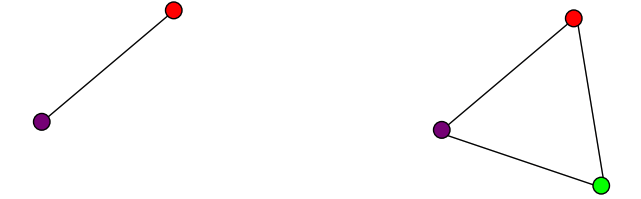
\includegraphics[width=10cm]{images/colour.png}
 \caption{Mixing two lights produces colours that lie along a straight line in colour space. Mixing three lights produces colours that lie within the triangle they define in colour space.}
\end{figure}

\subsubsection{RGB Space}
\begin{itemize}
 \item Primary colours are monochromatic lights (for monitors, they are the 3 types of phosphors used)
 \item Subtractive matching is required for certain wavelengths of light
\end{itemize}

\begin{figure}[H]
 \centering
 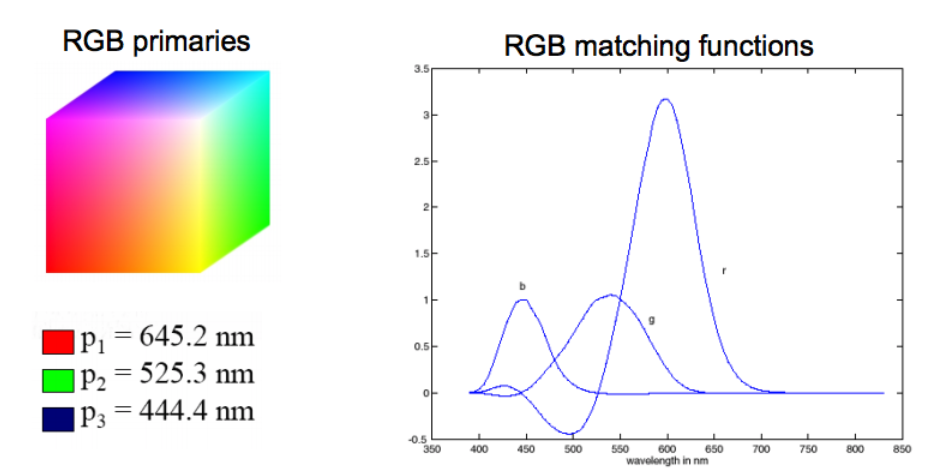
\includegraphics[width=10cm]{images/rgb.png}
 \caption{Representation of RBG primaries and corresponding matching functions. The matching functions are the amounts of primaries needed to match the monochromatic test color at the wavelength shown on the horizontal scale. Source: \url{https://en.wikipedia.org/wiki/CIE_1931_color_space}}
\end{figure}

\subsubsection{CIE XYZ Colour Space}
\begin{itemize}
 \item Primaries are imaginary, but matching functions are always positive
 \item The Y parameter corresponds to brightness or luminance of a colour
 \item Related to RGB space by linear transformation, upholding Grassman's Law
\end{itemize}
\begin{figure}[H]
 \centering
 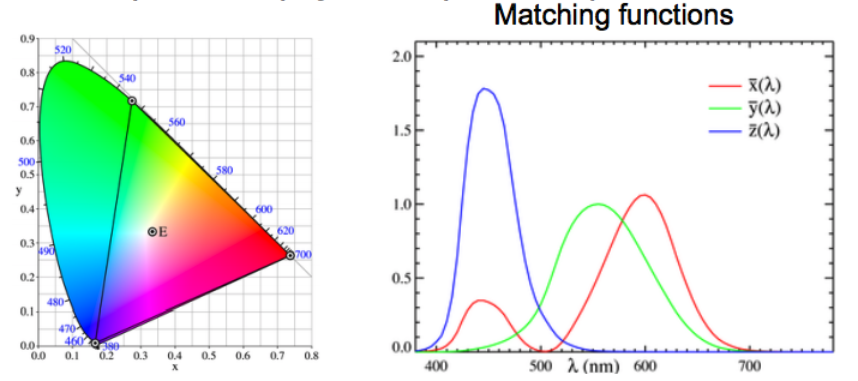
\includegraphics[width=10cm]{images/ciexyz.png}
 \caption{Source: \url{https://en.wikipedia.org/wiki/CIE_1931_color_space}}
\end{figure}


\subsubsection{Nonlinear Colour Spaces - HSV}
\begin{itemize}
 \item Designed to reflect more traditional and intuitive colour mixing models (ex. mixing paint)
 \item Based on how colours are used in human vision
 \item Dimensions are: Hue, Saturation, Value (intensity)
\end{itemize}
\begin{figure}[H]
 \centering
 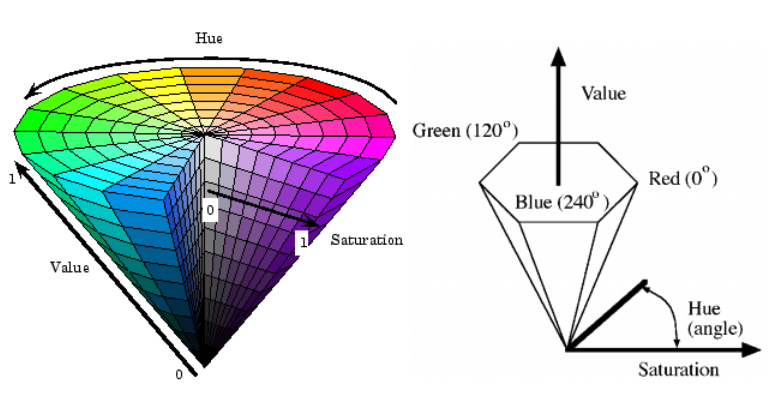
\includegraphics[width=10cm]{images/hsv.png}
 \caption{General source: \url{https://en.wikipedia.org/wiki/HSL_and_HSV}}
\end{figure}

\subsection{White Balancing}
\begin{description}
 \item[white balance]: process of adjusting image data captured by sensors to properly render neutral colours (white, gray, etc)
\end{description}
\begin{itemize}
 \item White balance adjustment performed automatically by digital cameras (custom settings for different lighting)
 \item Film cameras have different filters and film types for different conditions
\end{itemize}

\subsubsection{Importance of White Balancing}
\begin{itemize}
 \item White balancing is important because unadjusted images have an unnatural colour
       \begin{enumerate}
        \item Sensors in cameras or film are different from human eyes
        \item Different display media render images differently
        \item Viewing conditions when image was taken are usually different from image viewing conditions
       \end{enumerate}
\end{itemize}

\begin{figure}[H]
 \centering
 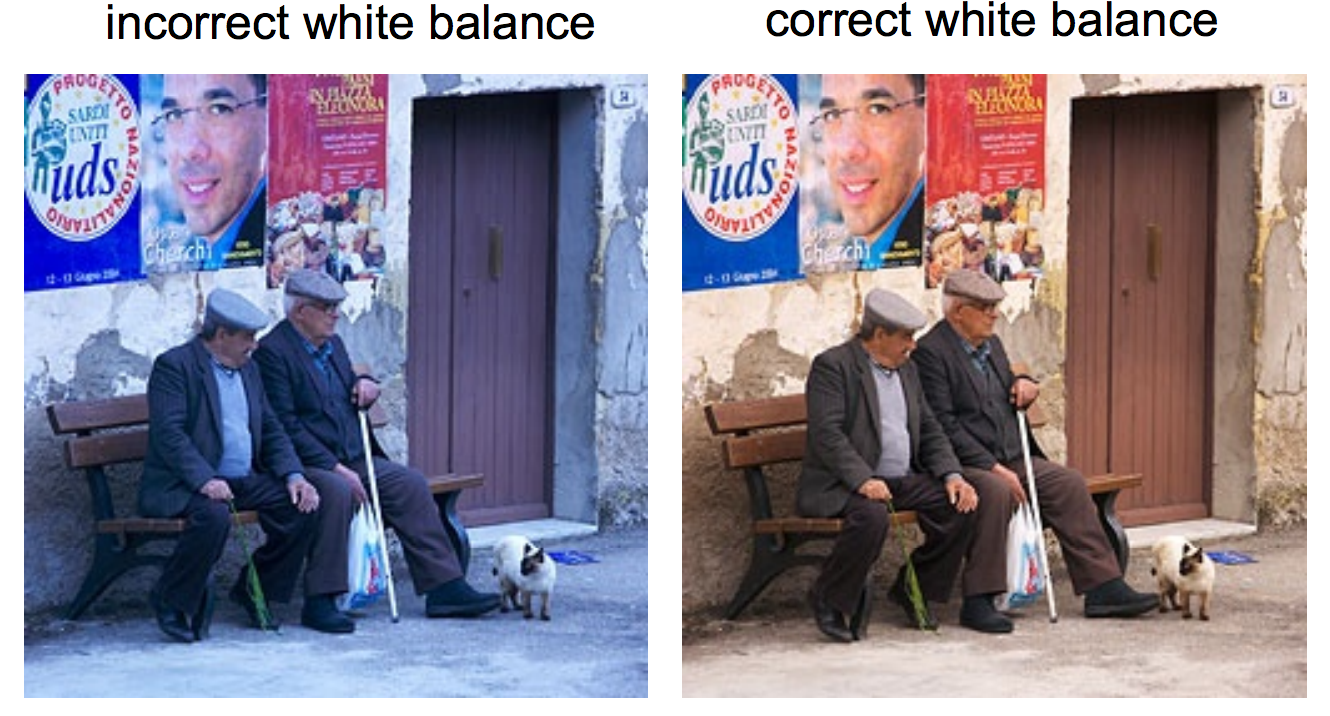
\includegraphics[width=10cm]{images/wb.png}
 \caption{Example of two photos, one unbalanced, and one with incorrect white balancing.  Source: \url{http://www.cambridgeincolour.com/tutorials/white-balance.htm}}
\end{figure}

\subsubsection{Von Kries Method}
\begin{description}
 \item[Von Kries method]: scale each colour channel by a ``gain factor'' to match appearnce of a gray neutral object. Accomplished by using the \textbf{gray card method}
 \item[Gray Card method]: take photo of neutral (gray or white) card and determine values of each channel. If we find that the card has RGB values $r_w$, $g_w$, $b_w$, then we scale each channel by $\frac{1}{r_w}$, $\frac{1}{g_w}$, $\frac{1}{b_w}$
\end{description}

\subsubsection{Other White Balancing Methods}
\begin{itemize}
 \item Without Gray Cards, we need to guess which pixels correspond with white objects
\end{itemize}
\begin{description}
 \item[Gray World Assumption]: assume that the average pixel value in the photo ($r_{avg}$, $g_{avg}$, $b_{avg}$) is gray and scale the image pixels by $\frac{1}{r_{avg}}$, $\frac{1}{g_{avg}}$, $\frac{1}{b_{avg}}$
 \item[Brightest Pixel Assumption]: apply a weighting to each channel that is inversely proportional to the values of the brightest pixels. Works on non-saturated images and assumes that image highlights usually have the colour of the light source (which is usually white)
 \item[Gamut Mapping]: apply a transformation to the image that maps the gamut of the image to the gamut of a "standard" image under white light
 \item[Gamut]: set of all pixel colours displayed in an image. In mathematical terms, this is a ``convex hull'' and a subset of all possible colour combintations
\end{description}


\subsection{Colour in Computer Vision}
\begin{itemize}
 \item Colour histograms for indexing and retrieval
 \item Skin detection
 \item Image segmentation and retrieval
 \item Buiilding appearance models for tracking
\end{itemize}

\section{Pixels and Filters}
\subsection{Images Types}
\begin{enumerate}
 \item Binary (black and white only)
 \item Greyscale
 \item Colour
\end{enumerate}

\subsubsection{Binary Image Representation}
\begin{itemize}
 \item Pixel values have an integer 0 or 1 value
       \begin{itemize}
        \item 0: black
        \item 1: white
       \end{itemize}
 \item Image is a 2D array of 0's and 1's
\end{itemize}

\subsubsection{Grayscale}
\begin{itemize}
 \item Pixel values have integer values in [0, 255] to represent a wider range of intensity
       \begin{itemize}
        \item 0: black
        \item 1 - 254: some shade of grey
        \item 255: white
       \end{itemize}
 \item Image is 2D array of integers in [0, 255]
\end{itemize}

\subsubsection{Colour Image}
\begin{itemize}
 \item 3 channels (RGB), each with integer values in [0, 255]
       \begin{itemize}
        \item 0: absence of primary
        \item 1 - 254: some contribution of primary
        \item 255: full contribution of primary
       \end{itemize}
 \item Image is a stack of 3 2D arrays of integers in [0, 255]
 \item i.e. 3 channels (RGB, LAB, HSV)
 \item Colour is represented with 3 numbers (3D coordinates in 3D colour space)
       \begin{itemize}
        \item RGB: [R, G, B]
        \item Lab: [L, a, b]
        \item HSV: [H, S, V]
       \end{itemize}
\end{itemize}

\subsection{Sampling and Resolution}
\begin{itemize}
 \item Images are \textbf{samples}; they are not continuous and consist of discrete pixels of a certain size and density
 \item Pixels have a nonzero size \lra images have limited resolution
 \item Fine details (smaller than pixel width) are approximated by pixels, which introduces \underline{error}
       \begin{description}
        \item[Resolution]: sampling parameter defined in dots per inch (DPI) or equivalent measures of spatial density. Standard screens have 72 DPI.
        \item[Pixels]: quantized to an integer value within [0,255]. Pixel value is in ``grayscale'' (or ``intensity'')
       \end{description}
\end{itemize}

\subsection{Image Histograms}
\begin{description}
 \item[Histogram]: provides frequency of brightness (intensity) values in the image (how many times a certain pixel value appears in the image). Captures the distribution of grey levels in the image (or color channel)
\end{description}
\begin{itemize}
 \item Histograms help us detect particular image features
       \begin{itemize}
        \item Sky: smooth coloration denotes consistency in image, consistent with the image of a sky
        \item Grass: a jagged histogram shows a wide ranging variety in colouration, consistent with the shadows in a grass field
        \item Faces: the colour composition of a face will be displayed in a histogram
       \end{itemize}
 \item Histograms can be used to provide a quantifiable description of what things look like; this can be used as input to classifiers
\end{itemize}

\begin{lstlisting}
  def histogram(im):
    for row in im.shape[0]:
      for col in im.shape[1]:
        val = im[row, col]
        h[val] += 1
\end{lstlisting}

\begin{figure}[H]
 \begin{center}
  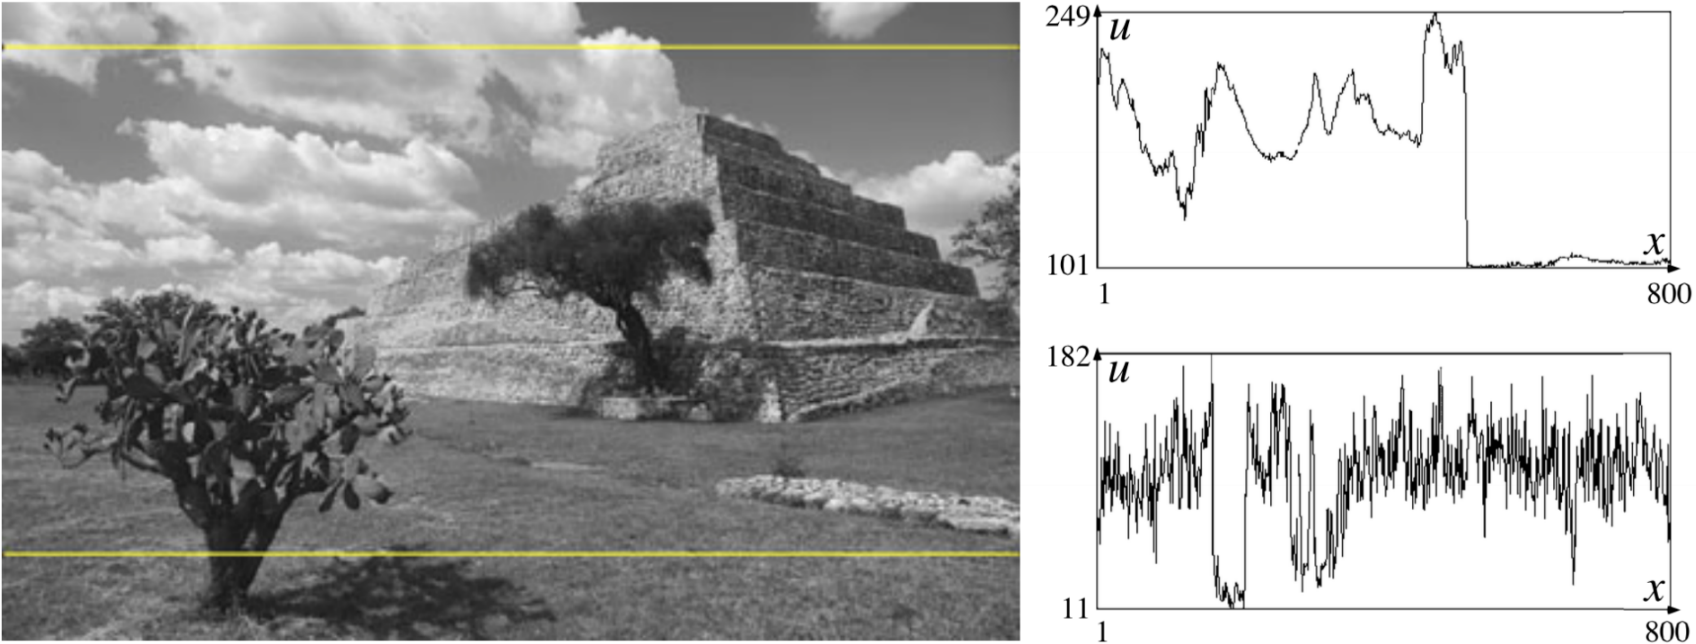
\includegraphics[scale=0.4]{images/histogram.png} \\
  \caption{The image is sampled at two vertical positions, sampling a patch of sky and sampling a patch of grass. The corresponding histograms are shown to the right. Adapted from the accompanying lecture slide (Slide 23, slide credit Dr. Mubarak Shah}
 \end{center}
\end{figure}

\subsection{Images as Functions}
\begin{itemize}
 \item Images are usually digital (discrete representations of the photographed scene)
 \item They sample the 2D space onto a regular grid to produce a representation of the image as a matrix of integer values
 \item When dealing with images, we can imagine the image matrix as infinitely tall and wide
       \begin{align}
        \begin{bmatrix}
         \ddots &           & \vdots   &          & \idots \\
                & f[-1, 1]  & f[0, 1]  & f[1, 1]           \\
         \dots  & f[-1, 0]  & f[0, 0]  & f[0, 1]  & \dots  \\
                & f[-1, -1] & f[0, -1] & f[1, -1] & \dots  \\
         \idots &           & \vdots   &          & \ddots
        \end{bmatrix}
       \end{align}
 \item However, the displayed image is only a finite subset of this infinite matrix
 \item Thus, we can describe images as coordinates in a matrix
\end{itemize}

\begin{itemize}
 \item An image can also be treated as a function $f: \mathbb{R}^2 \to \mathbb{R}^N$ where $f[m,n]$ is the intensity of a pixel at position $(m,n)$
 \item Note: we use square brackets, instead of usual parantheses, to denote discrete functions
 \item When we treat an image as a function, it is defined over a rectangle with finite range
 \item ex. the following function $f$ returns the (grayscale) intensity of a single pixel in an image located in the region $[a,b] \times [c,d]$
       \begin{align}
        f: [a,b] \times [c,d] \to [0,255] \tag{Grayscale Pixel Intensity}
       \end{align}
       \begin{description}
        \item[domain support]: the set of values $[a,b] \times [c,d]$ which contains all the values that are valid inputs to the function $f$
        \item[range]: the set [0,255] which defines the set of possible outputs
       \end{description}
 \item An image can also be treated a function mapping $\mathbb{R}^2 \to \mathbb{R}^3$
 \item ex. the RGB intensities of a given pixel can be written as the function $g$
       \begin{align}
        g[x, y] = \begin{bmatrix} r[x, y] \\ g[x, y] \\ b[x, y] \end{bmatrix} \tag{Color Pixel Intensity}
       \end{align}
 \item where $r,g,b: [a,b] \times [c,d] \to [0,255]$
\end{itemize}

\subsection{Linear Systems (Filters)}
\begin{description}
 \item[filtering]: forming a new image whose pixel values are transformed from original pixel values
\end{description}
\begin{enumerate}
 \item Denoising: removing salt and pepper noise
 \item Super resolution: blurry \lra super detailed
\end{enumerate}

\begin{description}
 \item[linear systems]: converts an input function $f[m,n]$ to an output (or response) function $g[m,n]$ where $m$, $n$ are the independent variables. For images, ($m$, $n$) correspond with spatial position in the image
 \item[system operator $\mathcal{S}$]: maps a member of the set of possible output $g[m,n]$ to a member of the set of possible inputs $f[m,n]$
       \begin{align}
        g      & = \mathcal{S}[f]                 \\
        g[n,m] & = \mathcal{S}\{f[n,m]\}          \\
        f[m,n] & \xrightarrow{\mathcal{S}} g[m,n]
       \end{align}
\end{description}

\subsubsection{Filter 1: Moving Average (Smoothing)}
\begin{description}
 \item[Moving Average]: sets the value of a pixel to be the average of its neigbouring pixels. (ex. the nine pixels in a $3 \times 3$ area, when applying a $3 \times 3$ filter)
       \begin{align}
        g[m,n] = \frac{1}{9} \sum\limits^1\limits_{i=-1} \sum\limits^1\limits_{j=-1} f[m-i, n-j] \tag{Weighted Average}
       \end{align}
\end{description}
\begin{itemize}
 \item The weighted average filter smoothes out sharper edges/features in the image, creating a blurred or smoothed effect
       \begin{align}
        h[m,n] = \frac{1}{9}
        \begin{bmatrix}
         1 & 1 & 1 \\
         1 & 1 & 1 \\
         1 & 1 & 1
        \end{bmatrix}
       \end{align}
 \item Note: moving average filter is linear and shift-invariant
\end{itemize}

\subsubsection{Filter 2: Image Segmentation}
\begin{description}
 \item[Image Segmentation]: based on simple threshold where the filter sets a pixel either to 255 (white) or 0 (black) depending on whether or not it meets the threshold $t$
       \begin{align}
        g[m, n] = \begin{cases} 255 & f[m, n] \geq t \\ 0 & \text{otherwise}\end{cases} \tag{Threshold}
       \end{align}
\end{description}
\begin{itemize}
 \item The basic image segmentation filter divides an image's pixels into binary black or white regions depending on whether $f[m, n] \geq t$
\end{itemize}

\subsection{Properties of Systems}
\begin{itemize}
 \item Here are some useful properties that a system may or may not possess
\end{itemize}

\subsubsection{Amplitude Properties}

\begin{enumerate}
 \item \textbf{Additivity}: A system is additive if it satisfies the equation
       \begin{align}
        \mathcal{S}[f_i[m, n] + f_j[m, n]] = \mathcal{S}[f_i[m, n]] + \mathcal{S}[f_j[m, n]]
       \end{align}
 \item \textbf{Homogeneity}: A system is homogeneous if it satisfies the equation
       \begin{align}
        \mathcal{S}[\alpha f_i[n, m]] = \alpha\mathcal{S}[f_i[n, m]
       \end{align}
 \item \textbf{Superposition}: A system has the property of superposition if it satisfies the equation
       \begin{align}
        \mathcal{S}[\alpha f_i[n, m]] + \beta f_j[n, m]] = \alpha\mathcal{S}[f_i[n, m]] + \beta\mathcal{S}f_j[n, m]]
       \end{align}
 \item \textbf{Stability}: A system is stable if it satisfies the inequality
       \begin{align}
        \abs{f[n, m}] \leq k \implies 	\abs{g[n, m]}  \leq ck \quad\quad\quad \text{for some $c$}
       \end{align}
 \item \textbf{Invertibility}: A system is invertible if it satisfies the equation
       \begin{align}
        \mathcal{S}^{-1}[\mathcal{S}[f[n, m]]] = f[n, m]
       \end{align}
\end{enumerate}

\subsubsection{Spatial Properties}
\begin{enumerate}
 \item \textbf{Causality}: A system is causal if for $m < m_0$ and $n < n_0$
       \begin{align}
        f[m, n] = 0 \implies g[m, n] = 0
       \end{align}
 \item \textbf{Shift Invariance}: A system is shift invariant if
       \begin{align}
        f[m - m_0, n - n_0] \xrightarrow{\mathcal{S}} g[m - m_0, n - n_0]
       \end{align}
\end{enumerate}

\subsection{Linear Systems}
\begin{description}
 \item[Linear system]: system that satisfies the property of superposition
 \item[Linear shift-invariant (LSI) system]: a linear system that is also shift-invariant
\end{description}
\begin{itemize}
 \item When we use a linear system for filtering, the new image pixels are weighted sums of the original pixel values, where the same set of weights are used for each pixel
 \item Note: Linear shift-invariant systems are important because human vision is linear shift-invariant
\end{itemize}

\subsubsection{Impulse Response}
\begin{itemize}
 \item To consider the impulse response of a system $\mathcal{S}$, pass the 2D delta function $\delta_2 [m,n]$ into the system
       \begin{align}
        \delta_2[m, n] = \begin{cases} 1 & m = 0 \text{ and } n = 0 \\
         0 & \text{otherwise}
        \end{cases}
       \end{align}
       \begin{description}
        \item[impulse response $h$]: by inputing the 2D delta function $\delta_2 [m,n]$ into the system, we get a filter $h[m,n]$ that tells us what the system is actually doing at each pixel
              \begin{align}
               h[m,n] = \mathcal{S}[\delta_2]
              \end{align}
       \end{description}
 \item Consider a $3 \times 3$ image $f[m,n]$
       \begin{align}
        f[m,n] =
        \begin{bmatrix}
         f[0,0] & f[0,1] & f[0,2] \\
         f[1,0] & f[1,1] & f[1,2] \\
         f[2,0] & f[2,1] & f[2,2] \\
        \end{bmatrix}
       \end{align}
 \item We can rewrite $f[m,n]$ as a sum of 2D delta functions
       \begin{align}
        f[m,n] & = f[0,0] \times \delta_2[m-0,n-0] + f[0,1] \times \delta_2[m-0,n-1] + \dots + f[m,n] \times \delta_2[0,0] + \dots \\
               & = \sum\limits_{i = -\infty}^{\infty}\sum\limits_{j = -\infty}^{\infty} f[i, j] \delta_2[m - i, n - j]
       \end{align}
 \item Now if we apply the system operator $\mathcal{S}$ to our image $f[m,n]$, we get
       \begin{align}
        \mathcal{S}[f[m,n]] & = \mathcal{S}\bigg[ \sum\limits_{i = -\infty}^{\infty}\sum\limits_{j = -\infty}^{\infty} f[i, j] \delta_2[m - i, n - j]  \bigg] \\
                            & = \sum\limits_{i = -\infty}^{\infty}\sum\limits_{j = -\infty}^{\infty} f[i, j] \mathcal{S} \bigg[ \delta_2[m - i, n - j] \bigg]
       \end{align}
 \item by applying superposition and shift invariance for $\mathcal{S}$
       \begin{align}
        \mathcal{S}[\alpha f_i[n, m]] + \beta f_j[n, m]] = \alpha\mathcal{S}[f_i[n, m]] + \beta\mathcal{S}f_j[n, m]]
       \end{align}
 \item Recall: the impulse response $h[m,n]$ is defined as $\mathcal{S}[\delta_2[m,n]]$, so
       \begin{align}
        f[m,n] = \sum\limits_{i = -\infty}^{\infty}\sum\limits_{j = -\infty}^{\infty} f[i, j] h[m-i,n-j]
       \end{align}
 \item Note: an LSI system is completely specified by its impulse response $h[m,n]$
       \begin{figure}[H]
        \begin{center}
         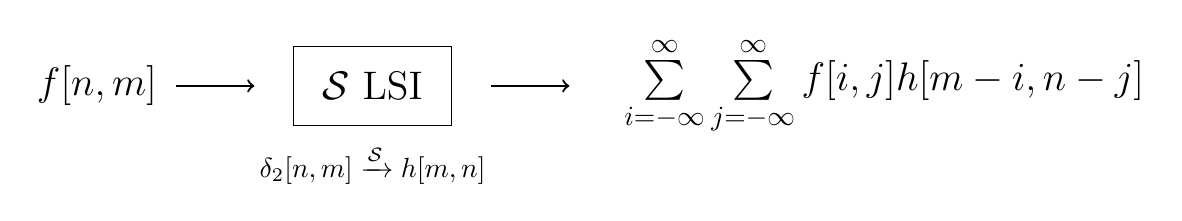
\begin{tikzpicture}
          \draw (-8, 0) node {\Large $f[n, m]$};
          \draw[->, thick] (-7, 0) -- (-6, 0);
          \draw (-5.5, 0.5) rectangle (-3.5, -0.5);
          \draw (-4.5, 0) node {\Large $\mathcal{S}$ LSI};
          \draw (-4.5,-1) node {$\delta_2[n,m] \xrightarrow{\mathcal{S}} h[m,n]$};
          \draw[->, thick] (-3, 0) -- (-2, 0);
          \draw (2, 0) node {\Large $\sum\limits_{i = -\infty}^{\infty}\sum\limits_{j = -\infty}^{\infty} f[i, j] h[m-i,n-j]$};
         \end{tikzpicture}
        \end{center}
        \caption{Graphical representation of the impulse response}
       \end{figure}
 \item Thus the impulse response $h[m,n]$ can be used to find the output image $g[m,n]$ with discrete convolution
       \begin{align}
        \mathcal{S}[f] = f[m,n] * h[m,n]
       \end{align}
\end{itemize}

\subsubsection{Impulse Response Example: Moving Average Filter}
\begin{itemize}
 \item The moving average filter is defined as
       \begin{align}
        g[m,n] = \frac{1}{9} \sum\limits^1\limits_{i=-1} \sum\limits^1\limits_{j=-1} f[m-i, n-j]
       \end{align}
 \item Using $h[m,n] = \mathcal{S}[\delta_2]$
       \begin{align}
        h[m,n] = \frac{1}{9} \sum\limits^1\limits_{i=-1} \sum\limits^1\limits_{j=-1} \delta_2[m-i, n-j]
       \end{align}
\end{itemize}


\subsection{Convolution}
\begin{description}
 \item[kernel $H$]: pattern of weights used for a linear filter
 \item[convolution]: process of applying the filter. Given a filter kernel $H$, the convolution of the kernel with image $F$ is an image $G$, where the $i,j$th component of $G$ is
       \begin{align}
        G = \sum\limits_{u}\sum\limits_{v} H_{i-u,j-v} F_{u,v}
       \end{align}
       \begin{itemize}
        \item Note: for convolution the kernel $H$ is flipped both horizontal and vertical direction (we have $-u$ and $-v$) before multiplying the overlapped input data $F$
       \end{itemize}
\end{description}
\begin{itemize}
 \item The easiest way to think of convolution is as a system that uses information from neighbouring pixels to filter the target pixel
 \item Convolution allows us to compute the output of passing any input signal through a system by simply considering the impulse response of the system
       \begin{itemize}
        \item This works because any signal can be decomposed into a weighted sum of impulse functions (ex. pixels in an image are 2D delta functions)
        \item This allows us to use the a weighted sum of the impulse responses for each part of the signal
       \end{itemize}
 \item The impulse response of a system, $h[n]$ is defined as the output resulting from passing an impulse function into a system
 \item When a system is linear, scaling the impulse function results in scaling of the impulse response by the same amount
 \item When a system is shift-invariant, shifting the impulse function shifts the impulse response by the same amount
 \item Thus, in general for an arbitrary input signal $x[n]= \sum\limits^{\infty}\limits_{k=-\infty} x[k] \delta [n-k]$ passed into a linear, shift-invariant system, the output is $y[n] = \sum\limits^{\infty}_{k=-\infty} x[h]h[n-k]$
       \begin{itemize}
        \item i.e the convolution of the signal $x$ with the impulse response $h$
       \end{itemize}
 \item 2D convolution is similar to 1D, but we have to iterate over 2 axes instead of 1
       \begin{align}
        f[m,n] * h[m,n] = \sum\limits_{i = -\infty}^{\infty}\sum\limits_{j = -\infty}^{\infty} f[i, j] h[m-i,n-j]
       \end{align}
 \item $f[m,n]*h[m,n]$ represents a function being multiplied by a shifted impulse response
 \item $f$ = image and $h$ = kernel
\end{itemize}

\subsubsection{2D Convolution Example: Identity Filter}
\begin{align}
 \begin{bmatrix}
  0 & 0 & 0 \\
  0 & 1 & 0 \\
  0 & 0 & 0
 \end{bmatrix}
 \tag{No change in output}
\end{align}

\subsubsection{2D Convolution Example: Shift Left Filter}
\begin{align}
 \begin{bmatrix}
  0 & 0 & 0 \\
  0 & 0 & 1 \\
  0 & 0 & 0
 \end{bmatrix}
 \tag{Shifts image left by 1 pixel}
\end{align}

\subsubsection{2D Convolution Example: Box Blur Filter}
\begin{align}
 \frac{1}{9}\begin{bmatrix}
  1 & 1 & 1 \\
  1 & 1 & 1 \\
  1 & 1 & 1
 \end{bmatrix}
 \tag{Blurs image}
\end{align}
\begin{itemize}
 \item The box blur filter takes the average of neighbouring pixels, which smoothes extreme features (less sharp)
\end{itemize}

\subsubsection{2D Convolution Example: Sharpening Filter}
\begin{align}
 \underbrace{\begin{bmatrix}
   0 & 0 & 0 \\
   0 & 2 & 0 \\
   0 & 0 & 0
  \end{bmatrix}
 -\frac{1}{9}\begin{bmatrix}
   1 & 1 & 1 \\
   1 & 1 & 1 \\
   1 & 1 & 1
  \end{bmatrix}}_\text{filter sums to 1} \\
 = \underbrace{\begin{bmatrix}
   0 & 0 & 0 \\
   0 & 1 & 0 \\
   0 & 0 & 0
  \end{bmatrix}}_\text{original image}
 +\underbrace{\begin{bmatrix}
   0 & 0 & 0 \\
   0 & 1 & 0 \\
   0 & 0 & 0
  \end{bmatrix}
  -\frac{1}{9}\begin{bmatrix}
   1 & 1 & 1 \\
   1 & 1 & 1 \\
   1 & 1 & 1
  \end{bmatrix}}_\text{details of the image}
 \tag{Blurs image}
\end{align}
\begin{itemize}
 \item By subtracting the average from the original picture, only the extreme features remain
 \item Adding the extreme features to the original image then accentuates differences (sharpens image)
\end{itemize}

\subsection{Implementation of Convolution: Image Support and Edge effects}
\begin{itemize}
 \item A computer will only compute finite support signals
 \item i.e. images that are zero for $m,n$ outside of rectangular region (the domain support)
 \item So convolution software often zero pads the matrix
 \item Numpy's convolution performs 2D discrete system convolution of finite support signals
 \item At the edge, can either do
       \begin{itemize}
        \item zero padding
        \item edge value replication
        \item mirror extension (wrap around to other side)
       \end{itemize}
\end{itemize}

\subsection{Cross Correlation **}
\begin{itemize}
 \item \textbf{Cross Correlation} of two 2D signals $f[m,n]$ and $g[m,n]$ is
       \begin{align}
        r_{fg}[k,l] & \triangleq \sum\limits^{\infty}\limits_{m=-\infty} \sum\limits^{\infty}\limits_{n=-\infty} f[m,n] * g[m-k, n-l]                       \\
                    & = \sum\limits^{\infty}\limits_{m=-\infty} \sum\limits^{\infty}\limits_{n=-\infty} f[m-k,n-l]g^{*}[m,n], \quad\quad k,l \in \mathbb{Z}
       \end{align}
 \item $(k,l)$ is called the \textbf{lag}
 \item Cross correlation is equivalent to convolution without the flip of the filter kernel
       \begin{align}
        r_{fg}[m,n] = f[m,n] * g^{*}[-m, -n]
       \end{align}
 \item Note: $g^{*}$ is defined as the complex conjugate of $g$. In this class, $g(n,m) \in \mathbb{R}$ so $g^{*} = g$
 \item Correlation can be used to find known features in images by using a kernel that contains target features
\end{itemize}

\subsubsection{Properties of Cross Correlation}
\begin{enumerate}
 \item \textbf{Associative property}:
       \begin{align}
        (f**h_1)**h_2 = f**(h_1 ** h_2)
       \end{align}
 \item \textbf{Distributive property}:
       \begin{align}
        f**(h_1 + h_2) = (f**h_1) + (f**h_2)
       \end{align}
 \item \textbf{Commutative property}:
       \begin{align}
        h_1 ** h_2 = h_2 ** h_1
       \end{align}
 \item \textbf{Shfit property}:
       \begin{align}
        f[m,n] ** \delta_2[m-m_0,n-n_0] = f[m-m_0,n-n_0]
       \end{align}
 \item \textbf{Shift invariance}:
       \begin{align}
        g[m,n]   & = f[m,n] ** h[m,n]                            \\
        \implies & f[m-\ell_1,n-\ell_l] ** h[m-\ell_2, n-\ell_2]
        = g[m-\ell_1 - \ell_2, n-\ell_1 -\ell_2]
       \end{align}
\end{enumerate}

\subsubsection{Convolution vs Cross Correlation}
\begin{itemize}
 \item Correlation is equivalent to convolution, i.e. $f**g = f*g$ \textbf{only} when the kernel/filter is \textbf{symmetric}
\end{itemize}
\begin{description}
 \item[Convolution]: integral that expresses the amount of overlap of one function as it is shifted over another function. Convolution is a \underline{filtering operation}
 \item[Correlation]: calculates a similarity measure for two input signals (ex. 2 image patches). The output of correlation reaches a maximum when the two signals match best. Correlation is a \underline{measure of relatedness} of two signals
\end{description}

\subsection{Discrete Convolution *}
\begin{itemize}
 \item Fold $h[k,l]$ about origin to form $h[-k,-l]$ (flip both horizontally and vertically)
 \item Shift the folded results by a number $k$ to form $h[m-k, n-\ell]$
 \item Multiply the kernel $h[m-k, n-\ell]$ by the image pixel $f[k,l]$
 \item Sum over all $k,\ell$
 \item Repeat for every number
\end{itemize}

\section{Edge Detection}
\begin{itemize}
 \item \textbf{Goal}: identify sudden changes (discontinuities) in an image
 \item Intuitively, most semantic and shape info from the image can be encoded in the edges
 \item Edge representation is more compact than pixels
 \item \textbf{Ideal}: artist's line drawing (but artist is also using object-level knowledge)
\end{itemize}

\subsubsection{Why are Edges Useful}
\begin{itemize}
 \item Extract info and recognize objects
 \item Recover geometry and viewpoints  (ex. vanishing lines)
\end{itemize}

\subsubsection{Origins of Edges in Images}
\begin{enumerate}
 \item Surface normal discontinuities
       \begin{itemize}
        \item ex. corners or edges where different planes intersect
        \item Each plane has a different normal and as you cross the corner/edge, the surface normal changes drastically resulting in an edge
       \end{itemize}
 \item Depth discontinuities
       \begin{itemize}
        \item Differences in depth results in different lighting and thus an image edge
       \end{itemize}
 \item Surface colour discontinuities
       \begin{itemize}
        \item ex. shadows, patterns on an object (ex. tiles)
       \end{itemize}
 \item Illumination discontinuity
\end{enumerate}
\begin{figure}[H]
 \centering
 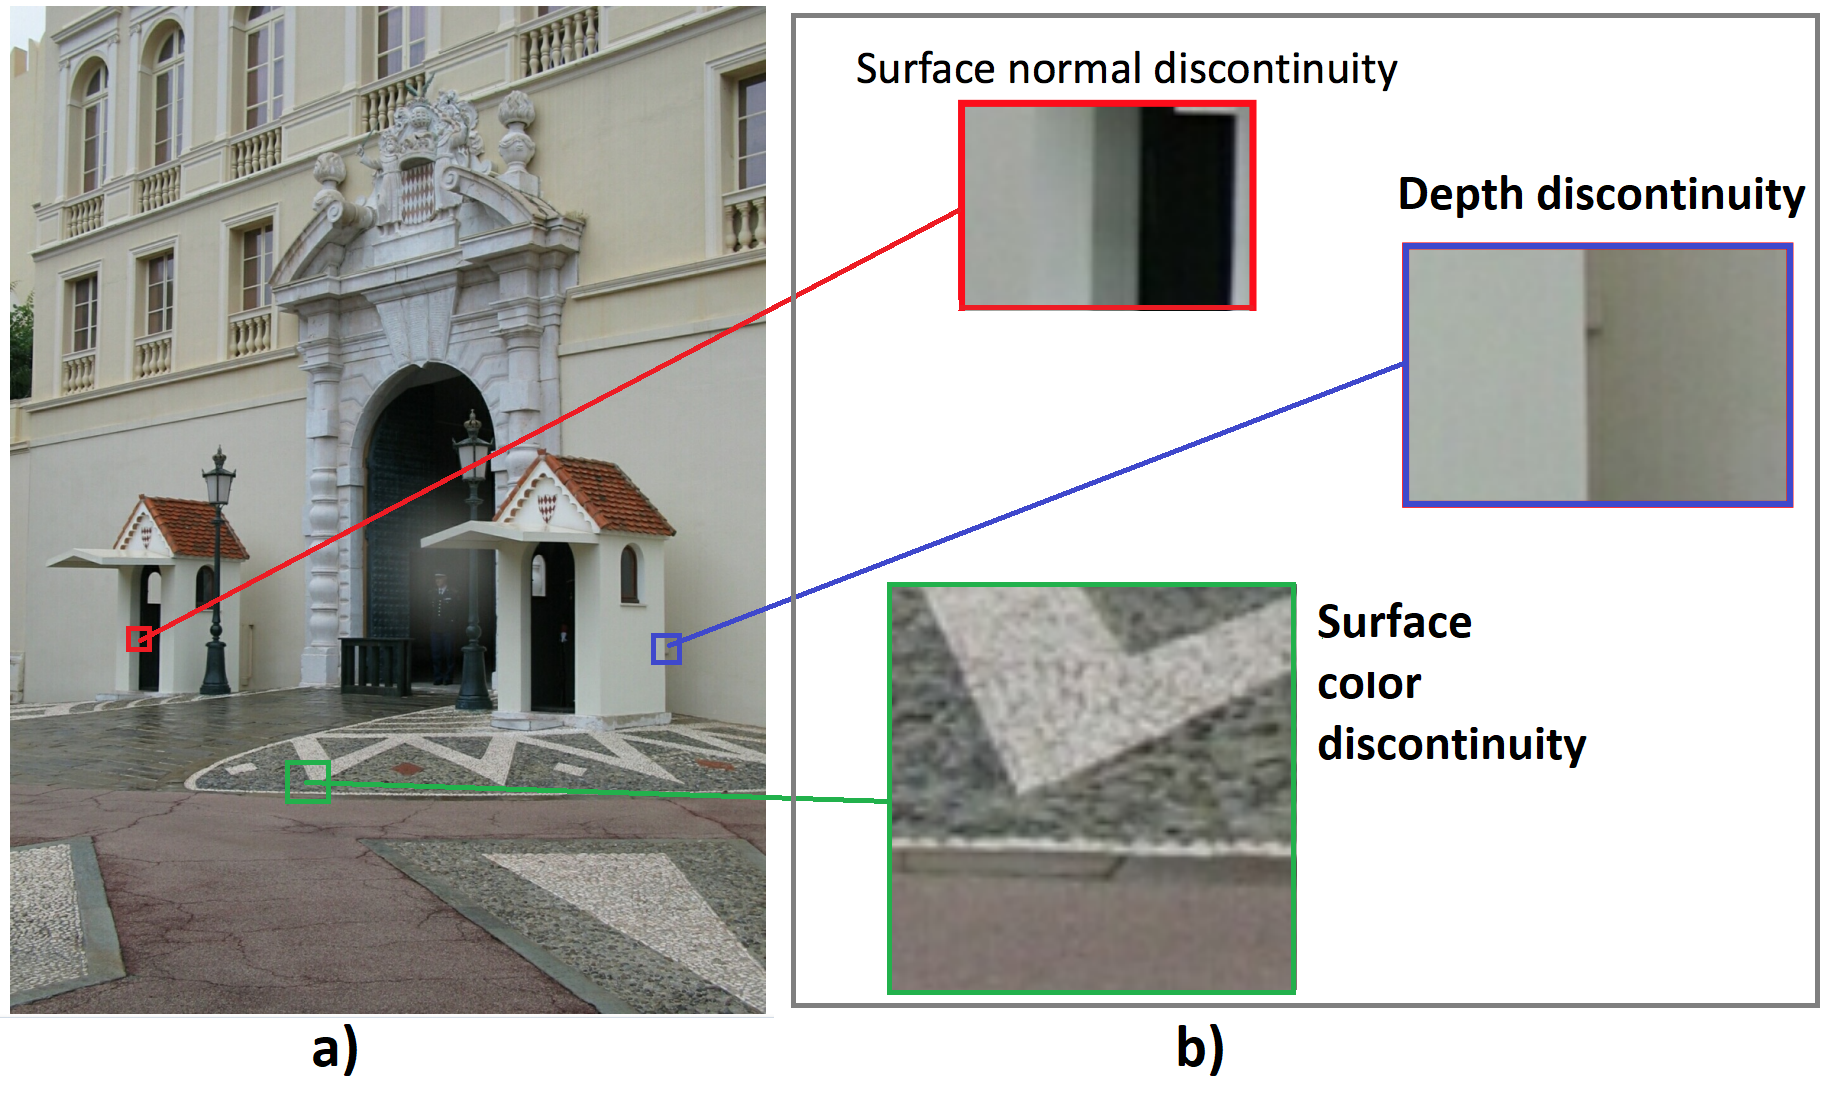
\includegraphics[width=8cm]{images/discontinuities.png}
 \caption{Examples of discontinities that create edges}
\end{figure}

\subsection{Image Gradients}
\subsubsection{1D Derivatives}
\begin{description}
 \item[Continuous]:
       \begin{align}
        \frac{df}{dx} = \lim_{\Delta x \to 0} \frac{f(x) - f(x-\Delta x)}{\Delta x} = f'(x) = f_x
       \end{align}
 \item[Discrete estimate (finite differences)]:
       \begin{align}
        \frac{df}{dx} \approx f(x) - f(x-1) = f'(x) = f_x
       \end{align}
\end{description}


\subsubsection{1D Discrete Derivatives and Filters}
\begin{itemize}
 \item Note: can calculate discrete derivatives by convolving differentiation kernels (remember to flip filters for convolution)
 \item Differentiation is linear and shift invariant
\end{itemize}
\begin{description}
 \item[Backward]:
       \begin{align}
        \frac{df}{dx} = f(x) - f(x-1) = f'(x)
       \end{align}
       \begin{align}
        \begin{bmatrix}
         0 & 1 & -1
        \end{bmatrix}
       \end{align}
 \item[Forward]:
       \begin{align}
        \frac{df}{dx} = f(x) - f(x+1) = f'(x)
       \end{align}
       \begin{align}
        \begin{bmatrix}
         -1 & 1 & 0
        \end{bmatrix}
       \end{align}
 \item[Central]:
       \begin{align}
        \frac{df}{dx} = f(x+1) - f(x-1) = f'(x)
       \end{align}
       \begin{align}
        \begin{bmatrix}
         1 & 0 & -1
        \end{bmatrix}
       \end{align}
\end{description}

\subsection{2D Continuous Derivatives}
\begin{description}
 \item[2D function]:
       \begin{align}
        f(x,y)
       \end{align}
 \item[Gradient vector]:
       \begin{align}
        \nabla f(x,y) =
        \begin{bmatrix}
         \dfrac{\partial f(x,y)}{\partial x} \\[3ex]
         \dfrac{\partial f(x,y)}{\partial y}
        \end{bmatrix}
        = \begin{bmatrix}
         f_x \\
         f_y
        \end{bmatrix}
       \end{align}
 \item[Gradient magnitude]:
       \begin{align}
        \abs{\nabla f(x,y)} = \sqrt{f_x^2 + f_y^2}
       \end{align}
 \item[Gradient direction]:
       \begin{align}
        \theta = \arctan\bigg(\frac{f_y}{f_x}\bigg)
       \end{align}
\end{description}
\begin{itemize}
 \item Note: gradient direction is largely independent of illumination intensity
\end{itemize}

\subsubsection{2D Discrete Gradients}

\begin{itemize}
 \item Can approximate gradient using neighbouring pixels based on central discrete derivative equation extended to 2D
       \begin{itemize}
        \item The gradient in the x-dir is then given by
              \begin{align}
               \frac{1}{3}\begin{bmatrix}
                1 & 0 & -1 \\
                1 & 0 & -1 \\
                1 & 0 & -1
               \end{bmatrix}
              \end{align}
        \item The gradient in the y-dir is given by
              \begin{align}
               \frac{1}{3}\begin{bmatrix}
                1  & 1  & 1  \\
                0  & 0  & 0  \\
                -1 & -1 & -1
               \end{bmatrix}
              \end{align}
       \end{itemize}
 \item Note: the x-direction gradient detects vertical edges while the y-direction gradient detects horizontal edges
 \item ex. the x and y gradients for an image $I$ can be found by convolution with the $3 \times 3$ kernels
       \begin{align}
        I_y =
        \begin{bmatrix}
         10 & 10 & 20 & 20 & 20 \\
         10 & 10 & 20 & 20 & 20 \\
         10 & 10 & 20 & 20 & 20 \\
         10 & 10 & 20 & 20 & 20 \\
         10 & 10 & 20 & 20 & 20 \\
        \end{bmatrix}
        * \frac{1}{3}\begin{bmatrix}
         1  & 1  & 1  \\
         0  & 0  & 0  \\
         -1 & -1 & -1
        \end{bmatrix}
        = \begin{bmatrix}
         0 & 0 & 0 & 0 & 0 \\
         0 & 0 & 0 & 0 & 0 \\
         0 & 0 & 0 & 0 & 0 \\
         0 & 0 & 0 & 0 & 0 \\
         0 & 0 & 0 & 0 & 0 \\
        \end{bmatrix}
       \end{align}
       \begin{align}
        I_x =
        \begin{bmatrix}
         10 & 10 & 20 & 20 & 20 \\
         10 & 10 & 20 & 20 & 20 \\
         10 & 10 & 20 & 20 & 20 \\
         10 & 10 & 20 & 20 & 20 \\
         10 & 10 & 20 & 20 & 20 \\
        \end{bmatrix}
        * \frac{1}{3}\begin{bmatrix}
         1 & 0 & -1 \\
         1 & 0 & -1 \\
         1 & 0 & -1
        \end{bmatrix}
        = \begin{bmatrix}
         0 & 0  & 0  & 0 & 0 \\
         0 & 10 & 10 & 0 & 0 \\
         0 & 10 & 10 & 0 & 0 \\
         0 & 10 & 10 & 0 & 0 \\
         0 & 0  & 0  & 0 & 0 \\
        \end{bmatrix}
       \end{align}
\end{itemize}

\subsection{Simple Edge Detection}
\begin{description}
 \item[edge]: set of points with rapid change in the image intensity function. Edges correspond with the extrema of the derivative of the image intensity function.
\end{description}
\begin{figure}[H]
 \centering
 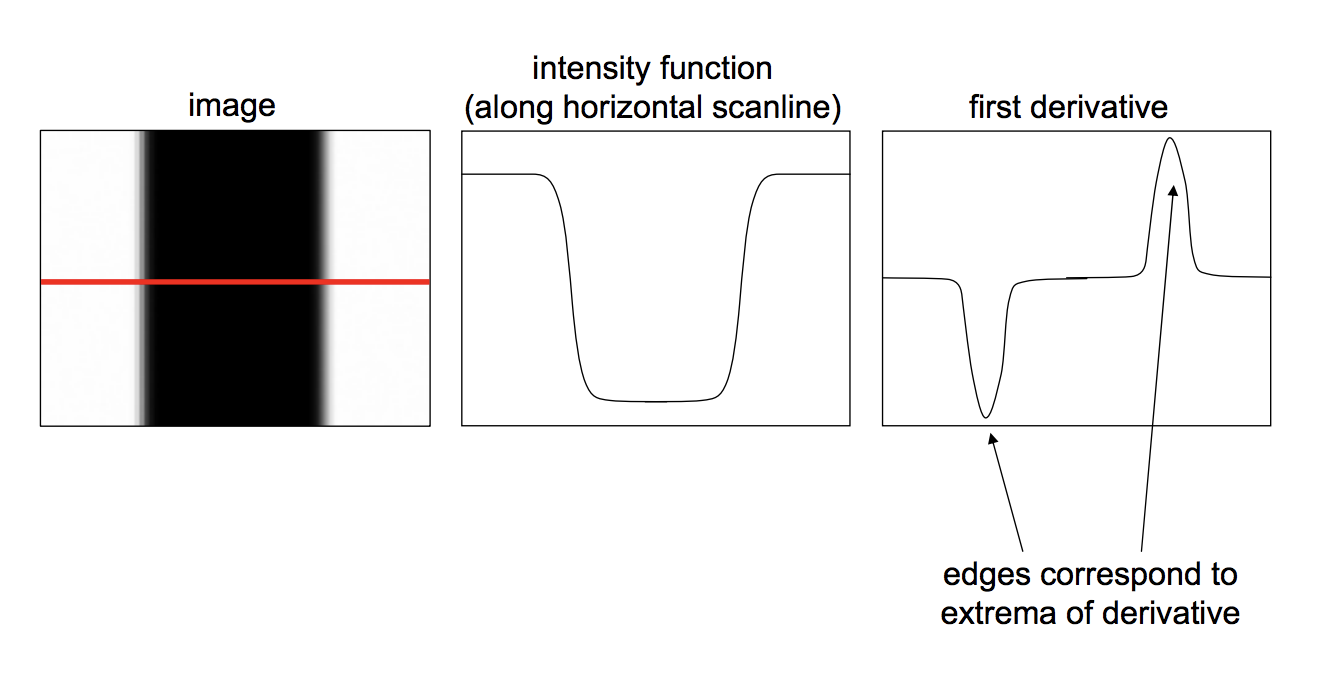
\includegraphics[height=6cm]{images/edge_intensity_extrema.png}
 \caption{An image with intensity function and first derivative}
\end{figure}

\subsubsection{Image Gradient}
\begin{description}
 \item[Gradient of an Image]: a vector that points in the direct of most rapid increase in intensity
       \begin{align}
        \nabla f =
        \begin{bmatrix}
         \dfrac{\partial f}{\partial x} \\[3ex]
         \dfrac{\partial f}{\partial y}
        \end{bmatrix}
       \end{align}
 \item[Gradient direction]:
       \begin{align}
        \theta = \arctan\bigg(\frac{f_y}{f_x}\bigg)
       \end{align}
 \item[Edge strength]: magnitude of image gradient
       \begin{align}
        \norm{\nabla f} = \sqrt{\bigg(\frac{\partial f}{\partial x}\bigg)^2 + \bigg(\frac{\partial f}{\partial y}\bigg)^2}
       \end{align}
\end{description}

\begin{figure}[H]
 \centering
 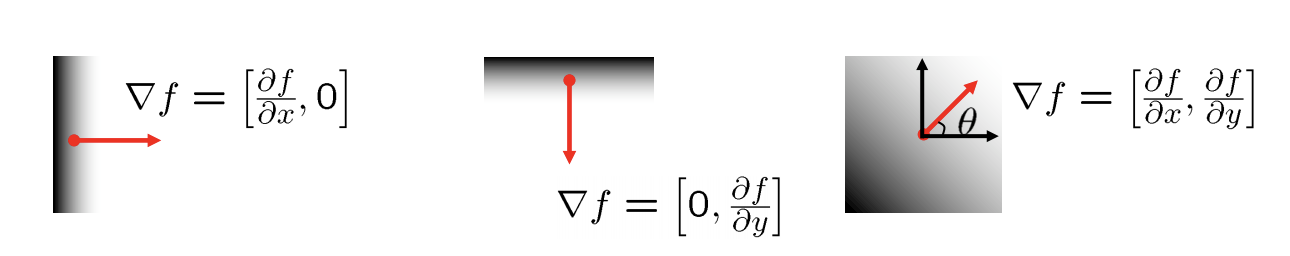
\includegraphics[width=10cm]{images/gradient_direction.png}
 \caption{The gradient vector directions}
\end{figure}

\begin{itemize}
 \item The shadows (dark spots) in an image derivative show which direction derivative you have
       \begin{itemize}
        \item vertical shadows \lra x-dir derivative
        \item horizontal shadows \lra y-dir derivative
       \end{itemize}
\end{itemize}

\begin{figure}[H]
 \centering
 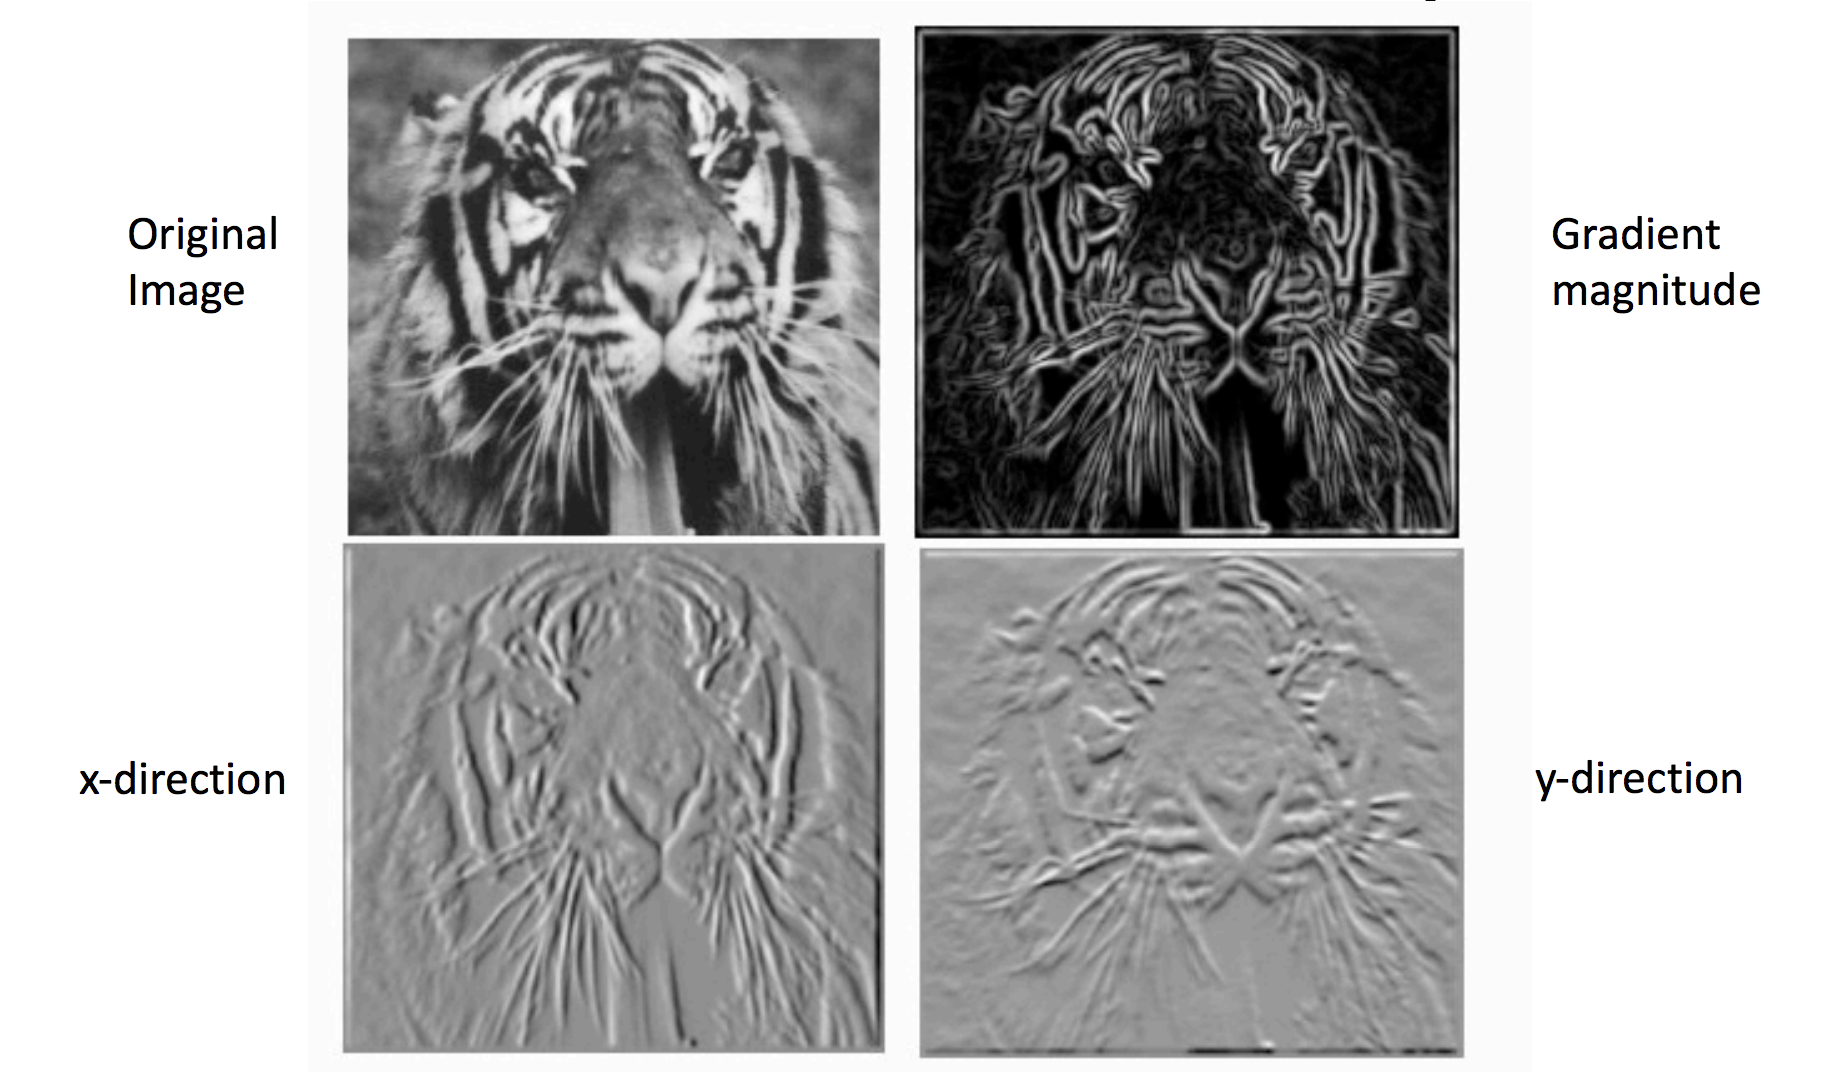
\includegraphics[width=10cm]{images/tiger_gradient.png}
 \caption{The gradients applied to an image of a tiger}
\end{figure}

\subsection{Intensity Profile}
\subsubsection{Effects of Noise}
\begin{itemize}
 \item With noise, it is hard to find the edge from maxima in derivative (because derivative is sensitive to noise and makes a lot of erroneous peaks)
 \item Finite difference filters respond strongly to noise
       \begin{itemize}
        \item Image noise results in pixels that look very different from their neighbours
        \item Generally, the larger the noise, the stronger the response
       \end{itemize}
 \item Solution: smoothing the image should help by forcing the pixels that look different to their neighbours (poteintally noise pixels) to look more like their neighbours
\end{itemize}

\begin{figure}[H]
 \centering
 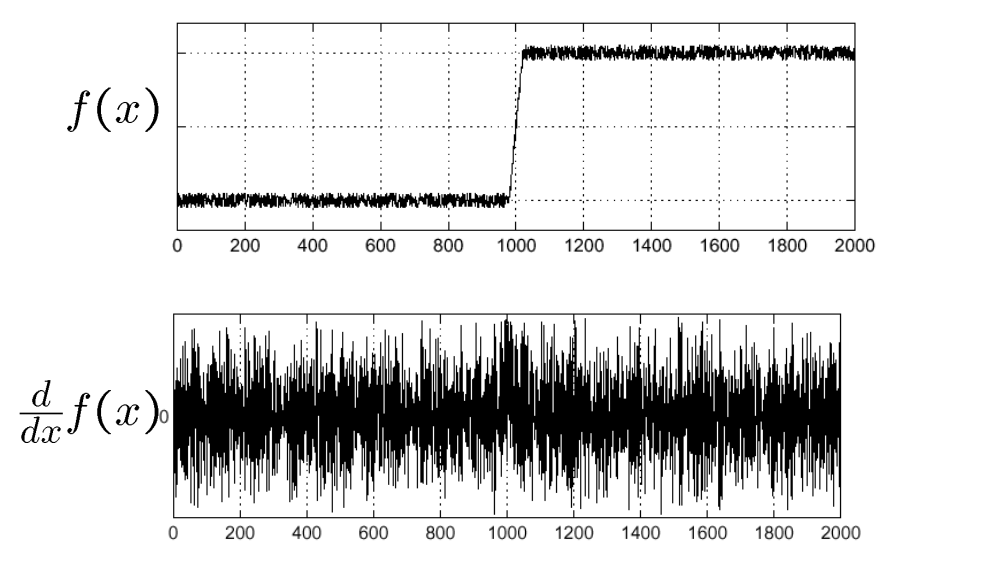
\includegraphics[width=10cm]{images/noisy_derivative.png}
 \caption{The derivative of an edge in a noisy image. Note it is extremely hard to find the edge with this noisy image}
\end{figure}

\subsubsection{1D Smoothing Filters}
\begin{description}
 \item[Mean smoothing filter]:
       \begin{align}
        \begin{bmatrix}
         1 \\
         1 \\
         1
        \end{bmatrix}
        \quad\quad\quad\quad
        \begin{bmatrix}
         1 & 1 & 1
        \end{bmatrix}
       \end{align}
 \item[Gaussian smoothing filter]:
       \begin{align}
        \begin{bmatrix}
         1 \\
         2 \\
         1
        \end{bmatrix}
        \quad\quad\quad\quad
        \begin{bmatrix}
         1 & 2 & 1
        \end{bmatrix}
       \end{align}
\end{description}

\subsubsection{Gaussian Blur}
\begin{description}
 \item[Gaussian blur]: blurring image with a Gaussian function to reduce image noise. Usually involves convolving with a filter that roughly approximates the 2D Gaussian
\end{description}
\begin{itemize}
 \item Note: Gaussian is a low-pass filter so it attenuates high frequency signals
 \item Gaussian blurring usually done as a preliminary step
\end{itemize}
\begin{description}
 \item[1D Gaussian]:
       \begin{align}
        G(x) = \frac{1}{\sqrt{2\pi\sigma}}e^{-\frac{x^2}{2\sigma^2}}
       \end{align}
 \item[2D Gaussian]:
       \begin{align}
        G(x,y) = \frac{1}{2\pi\sigma}e^{-\frac{x^2+y^2}{2\sigma^2}}
       \end{align}
\end{description}


\subsection{Smooth First Edge Detection (Unoptimized)}
\begin{figure}[H]
 \centering
 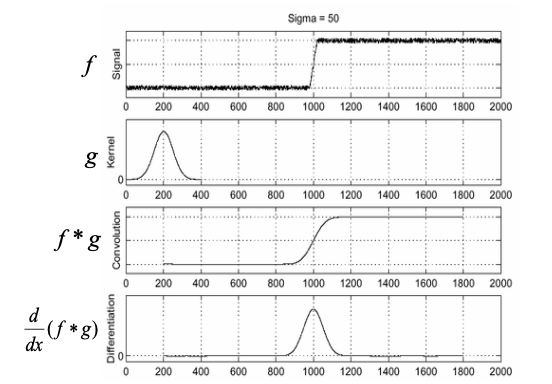
\includegraphics[width=10cm]{images/smooth_first_inefficient.png}
 \caption{Smooth first edge detection}
\end{figure}
\begin{itemize}
 \item To find edges, look for peaks in $\frac{d}{dx} (f*g)$
 \item Note: smoothing an image and then differentiating it is the same as convolving it with the derivative of a smoothing kernel
\end{itemize}

\subsubsection{Derivative Theorem of Convolution}
\begin{thm}{Derivative Theorem of Convolution}
 \begin{align}
  \frac{d}{dx} (f*g) = f*\frac{d}{dx} g
 \end{align}
\end{thm}
\begin{itemize}
 \item This allows us to save an extra step in edge detection
\end{itemize}

\subsubsection{Improved Smooth First Edge Detection}
\begin{figure}[H]
 \centering
 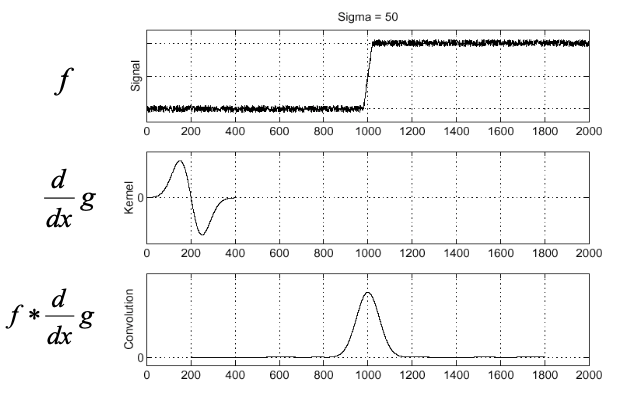
\includegraphics[width=10cm]{images/smooth_first_efficient.png}
 \caption{Improved smooth first edge detection}
\end{figure}

\subsection{Tradeoff between Smoothing at Different Scale $\sigma$}
\begin{itemize}
 \item Smoothed derivative reduces noise susceptibility but blurs edges
\end{itemize}

\subsection{Criteria for an Optimal Edge Detector}
\begin{enumerate}
 \item Good detection
       \begin{itemize}
        \item Minimizes probability of false positives (detecting fake edges caused by noise)
       \end{itemize}
 \item Good localization
       \begin{itemize}
        \item Detected edges must be as close as possible ot the true edges
       \end{itemize}
 \item Single response
       \begin{itemize}
        \item Detector must return one point only for each true edge point
        \item i.e. minimize the number of local maxima around the true edge
       \end{itemize}
\end{enumerate}
\begin{figure}[H]
 \centering
 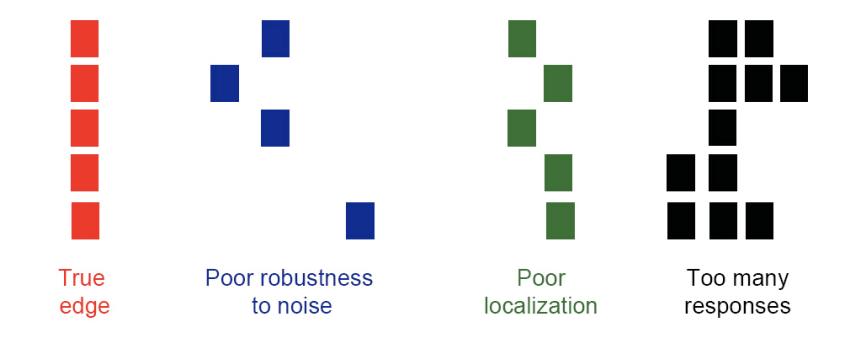
\includegraphics[width=8cm]{images/edge_detectors.png}
 \caption{Issues with bad edge detectors}
\end{figure}

\subsection{Sobel Edge Detector}
\begin{itemize}
 \item Uses two $3 \times 3$ kernels which are convolved with the original image to calculate approximations to the image gradient
 \item One kernel for horizontal changes and one for vertical
 \item Based on smoothing and differentiation idea
\end{itemize}

\subsubsection{Sobel Operator}
\begin{itemize}
 \item Note: Sobel kernels can be decomposed into a product of a smoothing and a differentiation kernel
\end{itemize}
\begin{description}
 \item[Sobel operator in x-dir $G_x$]:
       \begin{align}
        G_x = \begin{bmatrix}
         +1 & 0 & -1 \\
         2  & 0 & -2 \\
         +1 & 0 & -1
        \end{bmatrix}
        = \underbrace{\begin{bmatrix}
          1 \\
          2 \\
          1
         \end{bmatrix}}_\text{Gaussian smoothing}
        \underbrace{\begin{bmatrix}
          +1 & 0 & -1
         \end{bmatrix}}_\text{Differentiation}
       \end{align}
 \item[Sopel Operator in y-dir $G_y$]:
       \begin{align}
        G_x = \begin{bmatrix}
         +1 & +2 & +1 \\
         0  & 0  & 0  \\
         -1 & -2 & -1
        \end{bmatrix}
        =
        \underbrace{\begin{bmatrix}
          +1 \\
          0  \\
          -1
         \end{bmatrix}}_\text{Differentiation}
        \underbrace{\begin{bmatrix}
          1 & 2 & 1
         \end{bmatrix}}_\text{Gaussian smoothing}
       \end{align}
 \item[Sobel magnitude $G$]:
       \begin{align}
        G = \sqrt{G_x^2 + G_y^2}
       \end{align}
 \item[Angle/direction of gradient $\theta$]:
       \begin{align}
        \theta = \arctan\bigg(\frac{G_y}{G_x}\bigg)
       \end{align}
\end{description}

\subsubsection{Sobel Operator Issues}
\begin{enumerate}
 \item Poor localization
       \begin{itemize}
        \item Sobel operator triggers response in multiple adjacent pixels
       \end{itemize}
 \item Thresholding value favours certain directions of otehrs
       \begin{itemize}
        \item Can miss oblique edges more than horizontal/vertical edges
        \item False negatives
       \end{itemize}
\end{enumerate}

\subsection{Canny Edge Detector}
\begin{itemize}
 \item Most widely used edge detector in computer vision
 \item Thoretical model: step edges corrupted by additive Gaussian noise
 \item Canny shows that 1\textsuperscript{st} derivative of Gaussian closely approximates the operator that optimizes the product of signal-to-noise ratio and lcoalization
\end{itemize}

\subsubsection{Canny Edge Detector Features}
\begin{enumerate}
 \item Suppresses noise
 \item Computes gradient magnitude and direction
 \item Apply Non-Maximum suppression
       \begin{itemize}
        \item Assumes minimal response
       \end{itemize}
 \item Use hysteresis and connectivity analysis to detect edges
\end{enumerate}

\subsubsection{Non-Maximum Suppression}
\begin{itemize}
 \item This step makes sure that edges are specific
 \item Assume that edge occurs where gradient reaches a maximum
 \item Suppress non-maximizing gradient even if it passes threshold
 \item Round all gradient directions to the nearest $45^{\circ}$
\end{itemize}

\subsubsection{Removing Unnecessary Gradients}
\begin{itemize}
 \item $\norm{\nabla G}(x,y)$ is the gradient at each pixel
       \begin{align}
        M(x,y) = \begin{cases} \norm{\nabla G}(x,y) & \text{if} \norm{\nabla G}(x,y) \geq \norm{\nabla G}(x',y') \text{ and } \norm{\nabla G}(x,y) \geq \norm{\nabla G}(x'',y'') \\ 0 & \text{otherwise}\end{cases}
       \end{align}
 \item Note: $x'$ and $x''$ are the neighbours of $x$ along normal direction to an edge
\end{itemize}

\subsubsection{Hysteresis Thresholding}
\begin{itemize}
 \item Avoid streaks near threshold values
 \item Define 2 thresholds \textbf{low} and \textbf{high}
       \begin{itemize}
        \item If less than low \lra \textbf{not an edge}
        \item If greater than high \lra \textbf{strong edge}
        \item If between low and high \lra \textbf{weak edge}
       \end{itemize}
\end{itemize}
\begin{itemize}
 \item if gradient at a pixel is
       \begin{itemize}
        \item Above high \lra \textbf{strong edge pixel}
        \item Below low \lra \textbf{non-edge pixel}
        \item Between low and high
              \begin{itemize}
               \item if connected to a strong edge pixel or other pixels in between low and high \lra \textbf{edge-pixel}
              \end{itemize}
       \end{itemize}
 \item Use breath-first or depth-first search to find all the edges
\end{itemize}

\subsubsection{Canny Edge Detector Algorithm}
\begin{enumerate}
 \item Filter image with $x,$ derivatives of Gaussian
 \item Find magnitude and orientation of gradient
 \item Non-maximum suppression
       \begin{itemize}
        \item Thins multi-pixel wide ``ridges'' down to single pixel width
       \end{itemize}
 \item Thresholding and hysteresis
       \begin{itemize}
        \item Define 2 thresholds: low and high
        \item Use the high threshold to start edges and the low threshold to continue them
       \end{itemize}
\end{enumerate}

\subsection{Effect of Standard Deviation $\sigma$ (aka scale) in Gaussian Filter}
\begin{itemize}
 \item Large $\sigma$ detects large scale edges
 \item Small $\sigma$ detects fine features
\end{itemize}


\subsection{Hough Transform}
\begin{description}
 \item[Hough Transform (HT)]: detects location of lines in an image using parametrized equations
\end{description}
\begin{itemize}
 \item Caveat: Hough transform can only detect lines, circles, and other structures \textbf{only} if their parametric equation is known
 \item Can give robust detection under noise and partial occlusion
\end{itemize}

\subsubsection{Preparation before applying Hough Transform}
\begin{itemize}
 \item Perform some edge detection and a thresholding of the edge magnitude
 \item Thus we have some pixels that may partially describe the boundary of some objects
\end{itemize}

\subsubsection{Detecting Lines using Hough Transform}
\begin{itemize}
 \item Goal: find sets of pixels that make up straight lines
 \item Consider a point of known coordinates $(x_i,y_i)$
 \item There are many lines passing through the point $(x_i, y_i)$
 \item Straight lines that pass through $(x_i, y_i)$ have the equation $y = ax_i + b$ for some set of parameters $(a,b)$
 \item We can rewrite this equation as $b = -ax_1 + y_1$ and consider $x,y$ as parameters and $a,b$ as variables
 \item This gives a line in $(a,b)$ space parametrixed in $x$ only
 \item Thus a single point in $(x_1,y_1)$ space gives us a line in $(a,b)$ space
 \item 2 points $(x_1,y_1)$ and $(x_2,y_2)$ define a line in $(x,y)$ plane and also give rise to 2 diferent liens in $(a,b)$ space
 \item In $(a,b)$ space, these lines will intersect at $(a',b')$
 \item Thus, all points on the line defined by $(x_1,y_1)$ and $(x_2,y_2)$ in $(x,y)$ space will parametrize liens that interesect in $(a',b')$ in $(a,b)$ space
\end{itemize}
\begin{figure}[H]
 \centering
 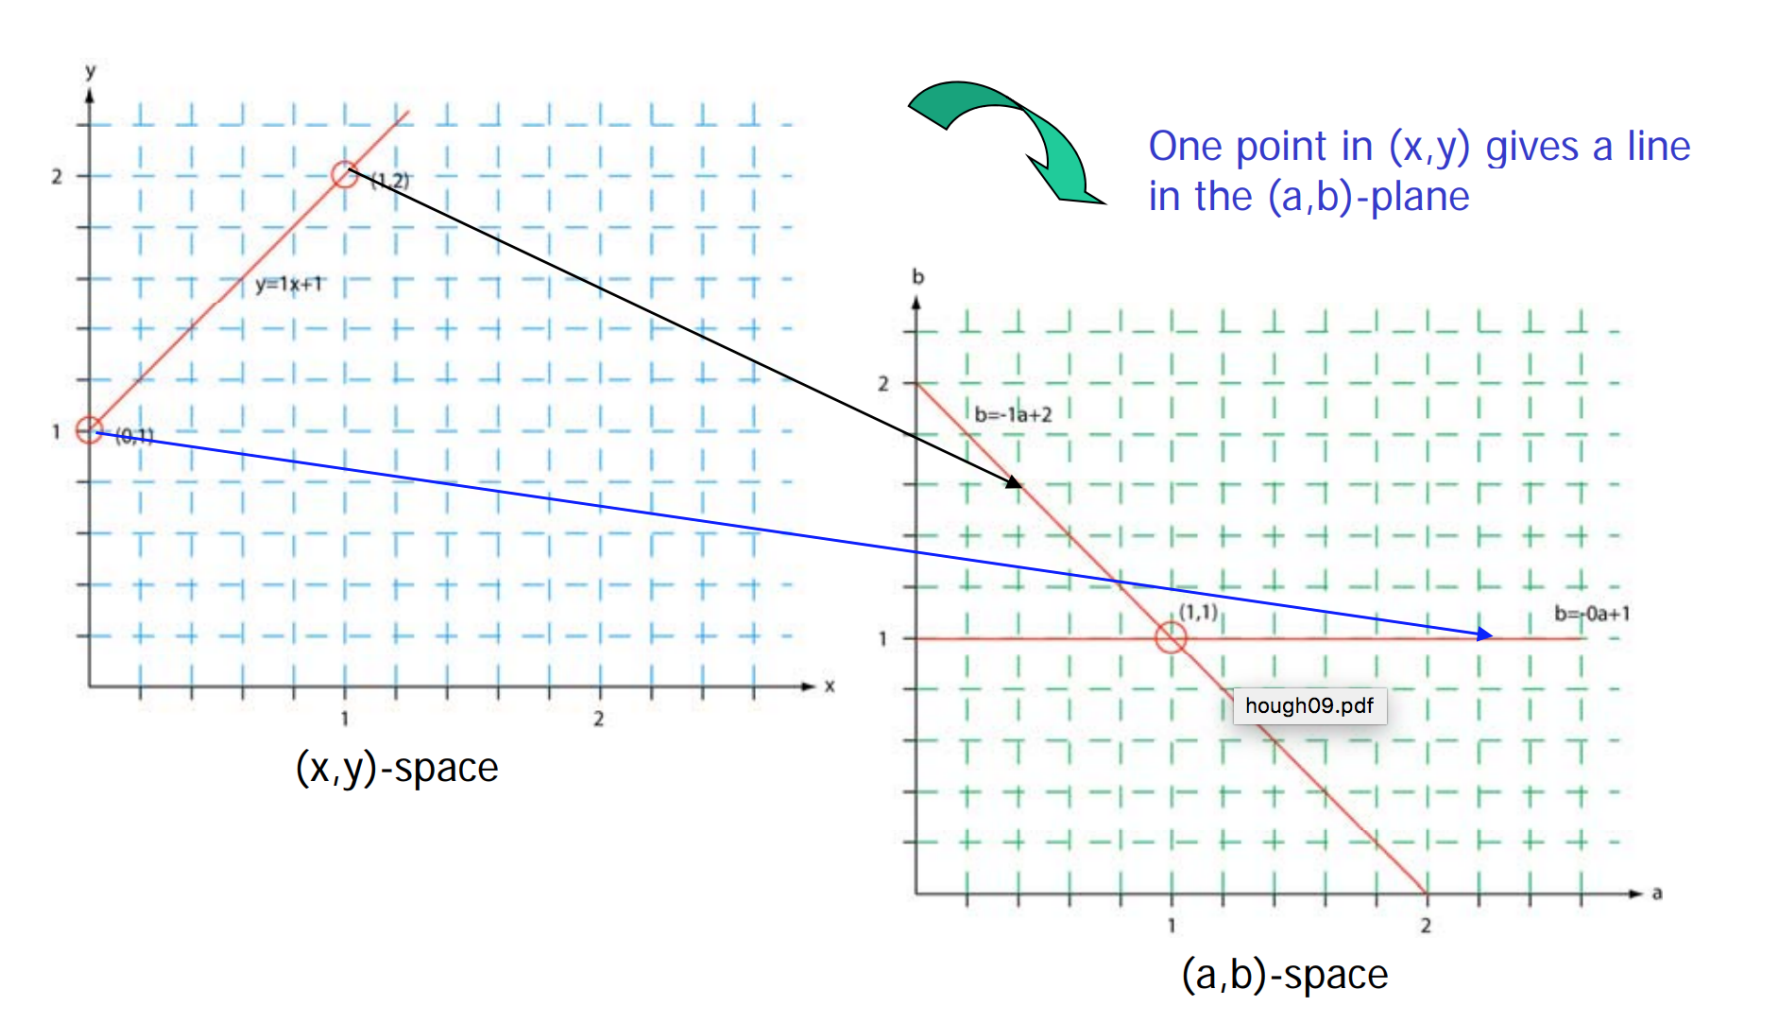
\includegraphics[width=\textwidth]{images/hough_transform.png}
 \caption{Transformation from original $(x,y)$ space to Hough $(a,b)$ space. Here we have two points $(x_1,y_1)=(1,1)$ and $(x_2,y_2)=(2,3)$. We transform these points into $(a,b)$ space to get the lines $b=-a*1 +1$ and $b=-a*2+3$. These two lines intersect at $a=2$ and $b=-1$, which gives us the equation for the original line in $(x,y)$ space as $y=2x-1$}
\end{figure}

\subsubsection{Hough Transform Algorithm}
\begin{enumerate}
 \item Quantize parameter space $(a,b)$ by dividing it into \textbf{accumulator cells}
 \item Count the number of times a line intersects a given cell
       \begin{itemize}
        \item For each pair of points $(x_1,y_1)$ and $(x_2,y_2)$ detected as an edge, find the intersection $(a',b')$ in $(a,b)$ space
        \item Increase the value of a cell in the range $[[a[[a_{min}, a_{max}],[b_{min},b_{max}]]$ that $(a', b')$ belongs to
       \end{itemize}
 \item Cells receiving more than a certain number of counts (aka \textbf{votes}) are assumed to correspond with lines in $(x,y)$ space
\end{enumerate}

\subsubsection{Hough Transform in $(\rho, \theta)$ space)}
\begin{itemize}
 \item Can represent lines as polar coordinates instead of $y=ax + b$ *allows us to represent vertical lines
       \begin{itemize}
        \item A vertical line will have $\theta=0$ and $\rho$ equal to the x-intercept
        \item A horizontal line will have $\theta=90$ and $\rho$ equal to the y-intercept
       \end{itemize}
       \begin{description}
        \item[Polar coordinate representation]: For a pixel $(x_i,y_i)$, we transform it with the equation $x\cos\theta + y\sin\theta = \rho$
       \end{description}
 \item Note: lines in $(x,y)$ space are sine wave-like functions in $(\rho, \theta)$ space
       \begin{figure}[H]
        \centering
        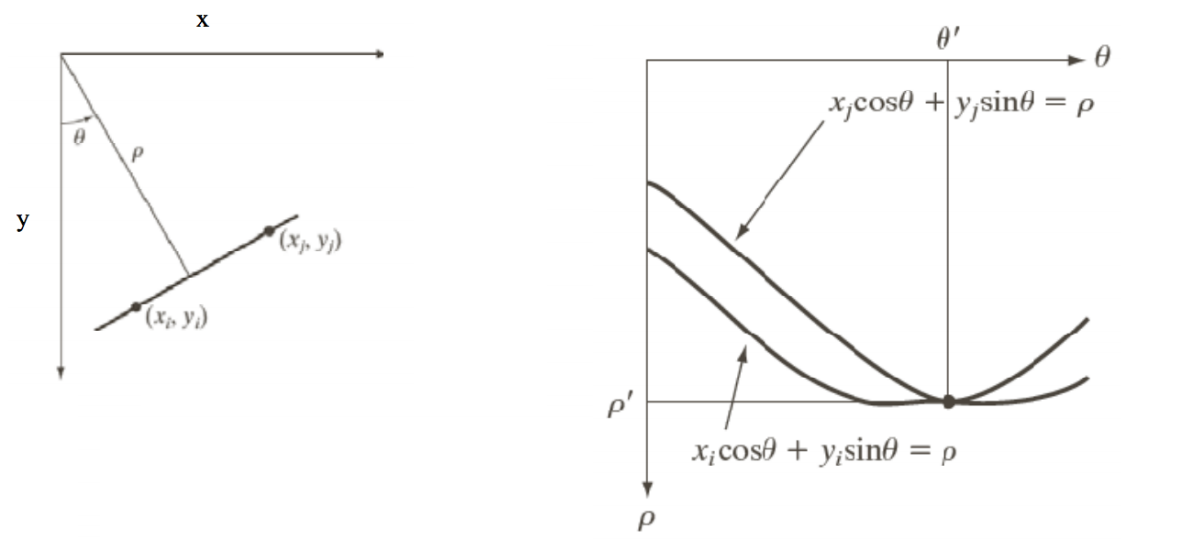
\includegraphics[width=\textwidth]{images/hough_transform_rho_theta.png}
        \caption{Transformation from original $(x,y)$ space to Hough $(\rho,\theta)$ space}
       \end{figure}
 \item Still use regular Hough Transform algorithm by looking for intersections of these transformed functions in $(\rho, \theta)$ space to get the $\rho,\theta$ parameter values
 \item Again, the accumulator cells with the most votes are most likely the real lines in our image
\end{itemize}

\subsubsection{Hough Transform Advantages}
\begin{itemize}
 \item Conceptually simple
 \item Easy implementation
 \item handles missing and occluded data very gracefully
 \item Can be adapted to many types of forms, not just lines
\end{itemize}

\subsubsection{Hough Transform Disadvantages}
\begin{itemize}
 \item Computational complex for objects with many parameters
 \item Looks for only one single type of object
 \item Can be ``fooled'' by ``apparent edges''
 \item Length and position of a line segment cannot be determined
 \item Co-linear segments cannot be separated
\end{itemize}














\end{document}
